% Complete Global Economy notes
% Set up for pdflatex

% sets formatting parameters etc
\documentclass[8pt,twoside,pdftex]{book}

% nice book overview: http://www.math.mun.ca/~edgar/thesis.html
% see esp indexing w/ package makeidx
% more at:  http://en.wikibooks.org/wiki/LaTeX/Indexing

\usepackage{amsmath, amssymb, amsthm}
\usepackage{graphicx}
\usepackage{color}
\usepackage{comment}
\usepackage{layout}
\usepackage{booktabs}
\usepackage{caption}
\usepackage{setspace}
\usepackage{float}

% link colors etc:  black for Amazon, blue for the online version
\usepackage[colorlinks=true,
            allcolors=blue,
%            linkcolor=black,
%            citecolor=black,
%            urlcolor=blue,
            bookmarks=false,
            pdfstartview={FitV},
            pdftitle={The Global Economy},
            pdfsubject={A course in macroeconomics for business students},
            pdfauthor={The NYU Stern Economics Team}
            ]{hyperref}

% Adjust fonts for chapter and section headings
% old version
\usepackage[medium, compact]{titlesec}
\titleformat{\section}{\large\bfseries}{\thesection}{1em}{}
\titleformat{\subsection}{\normalsize\bfseries}{\thesection}{1em}{}

% LC  version
%\usepackage[medium, compact, sf, bf]{titlesec} % edited by LC
%\titleformat{\section}{\large\bfseries\sffamily}{\thesection}{1em}{}  % edited by LC
%\titleformat{\subsection}{\normalsize\bfseries\sffamily}{\thesection}{1em}{}  % edited by LC
%\titleformat{\part}{\bfseries\huge\sffamily\uppercase}{}{0pt}{Part \thepart\\}  % edited by LC
%\titleformat{\chapter}{\bfseries\huge\sffamily\uppercase}{}{0pt}
%        {\ifnum\thechapter>0\resizebox{!}{30pt}{\thechapter}\\ \fi}  % edited by LC

% to kill off awkward pagebreaks
\usepackage{needspace}
% example:  \needspace{4\baselineskip} makes sure we have four lines available before pagebreak

% for left spacing of problems, summary, etc
\newlength{\oldleftmargini}
\setlength{\oldleftmargini}{\leftmargini}
% use these commands:
%\setlength{\leftmargini}{.5\oldleftmargini}
%\setlength{\leftmargini}{\oldleftmargini}

% for spacing of table of contents
% see http://tex.stackexchange.com/questions/49877/table-of-contents-spacing
% problem:  messes up spacing and fonts of table and figure lists in toc, so killed them off
\usepackage{tocloft}
\renewcommand\cftchapafterpnum{\vskip10pt}

%%%%%%%%%%%%%%%%%%%%%%Margins%%%%%%%%%%%%%%%%%%%%%%%%%%%%%%%%%%%%%%%%%%%%%%%
% http://en.wikibooks.org/wiki/LaTeX/Page_Layout
\usepackage{geometry}
\geometry{paperwidth=6in, paperheight=9in, outer=0.6in, inner=0.85in, bottom=0.6in}
%\usepackage[cam,letter,center,pdftex]{crop}

% indentation and para skips
\setlength{\parindent}{0in}
\setlength{\parskip}{\bigskipamount}  % this is diddled further in the front_matter
\raggedbottom

%%%%%%%%%%%%%%%%%%%%Tighten up the lists%%%%%%%%%%%%%%%%%%%%%%%%%%%%%%%%%%
\let\OLDdescription\description
\renewcommand\description{\OLDdescription\setlength{\itemsep}{-2mm}}

%%%%%%%%%%%%%%%%%%%%%%Headers and Footers%%%%%%%%%%%%%%%%%%%%%%%%%%%%%%%%%%
\usepackage{fancyhdr}
\pagestyle{fancy}
\fancyhead{}
\fancyfoot{}
\renewcommand{\chaptermark}[1]{\markboth{\thechapter.\ #1}{}}
\fancyhead[RO]{\leftmark \hspace{0.25in} \thepage}
\fancyhead[RE]{}
\fancyhead[LE]{\thepage \hfill Global Economy @ NYU Stern}

%%%%%%%%%%%%%%%%%%%%%%Special Characters%%%%%%%%%%%%%%%%%%%%%%%%%%%%%%%%%%%%
\newcommand{\GDP}{\mbox{\em GDP\/}}
\newcommand{\NDP}{\mbox{\em NDP\/}}
\newcommand{\GNP}{\mbox{\em GNP\/}}
\newcommand{\NX}{\mbox{\em NX\/}}
\newcommand{\NY}{\mbox{\em NY\/}}
\newcommand{\CA}{\mbox{\em CA\/}}
\newcommand{\NFA}{\mbox{\em NFA\/}}

\newcommand{\Def}{\mbox{\em Def\/}}
\newcommand{\DS}{\mbox{\em DS\/}}
\newcommand{\CPI}{\mbox{\em CPI\/}}
\newcommand{\POP}{\mbox{\em POP\/}}
\newcommand{\CU}{\mbox{\em CU\/}}
\newcommand{\RE}{\mbox{\em RE\/}}
\newcommand{\MB}{\mbox{\em MB\/}}
\newcommand{\MONE}{\mbox{\em M1\/}}
\newcommand{\MTWO}{\mbox{\em M2\/}}
\newcommand{\IP}{\mbox{\em IP\/}}
\newcommand{\RER}{\mbox{\em RER\/}}




%%%%%%%%%%%%%%%%%%%%%%%%%%%%%%%%%%%%%%%%%%%%%%%%%%%%%%%%%%%%%%%%%%%%%%%%%%%%%%%%%%%%%%%%%%%%%%%%%%%%
%To create a single chapter with the correct page numbering and references:                        %
%This isn't elegant, if you know a better way to do this, tell me.                                 %
%                                                                                                  %
% 1.  Go into preamble and set bookmarks=false.                                                    %
% 2.  Compile the entire book                                                                      %
% 3.  Uncomment the appropriate "includeonly" statement.                                           %
% 4.  The pdf will still be called "The_Global_Economy," so save it with the right filename.       %
% 5.  Some chapters may have a blank page at the beginning.  Use Acrobat to delete it.             %
%                                                                                                  %
%\includeonly{a_notes_front_matter}                                                                %
%\includeonly{notes_math}                                                                          %
%\includeonly{notes_data}                                                                          %
%\includeonly{notes_review_long}                                                                   %
%\includeonly{notes_production}                                                                    %
%\includeonly{notes_solow}                                                                         %
%\includeonly{notes_growth}                                                                        %
%\includeonly{notes_institutions}                                                                  %
%\includeonly{notes_finance}                                                                       %
%\includeonly{notes_trade}                                                                         %
%\includeonly{notes_labor}                                                                         %
%\includeonly{notes_review_short}                                                                  %
%\includeonly{notes_cycles}                                                                        %
%\includeonly{notes_indicators}                                                                    %
%\includeonly{notes_inflation}                                                                     %
%\includeonly{notes_asad}                                                                          %
%\includeonly{notes_asadpolicy}                                                                    %
%\includeonly{notes_monpol}                                                                        %
%\includeonly{notes_taxes}                                                                         %
%\includeonly{notes_deficits}                                                                      %
%\includeonly{notes_bop}                                                                           %
%\includeonly{notes_fx}                                                                            %
%\includeonly{notes_fxregimes}                                                                     %
%\includeonly{notes_crises}                                                                        %
%%%%%%%%%%%%%%%%%%%%%%%%%%%%%%%%%%%%%%%%%%%%%%%%%%%%%%%%%%%%%%%%%%%%%%%%%%%%%%%%%%%%%%%%%%%%%%%%%%%%


\begin{document}

%Title page, tables of contents, figures, etc.
\frontmatter
%%%%%%%%%%%%%%%%%%%%%%%%%%%%%%%%%%%%%%%%%%%%%%%%%%%%%%%%%Front Matter%%%%%%%%%%%%%%%%%%%%%%%%%%%%%%%%%%%%%%%
\begin{titlepage}
%\pagenumbering{roman}

\begin{center}
\textsc{}\\[1.5in]
{\Huge\bf The Global Economy} \\ [0.5in]
%\vfill
%{\includegraphics[width=0.65\textwidth]{Figures/stern_logo3.pdf}\\
%\textsc{\large Department of Economics}\\[1.5in]
%}
\end{center}

\pagebreak
\phantom{x}
\thispagestyle{empty}

\pagebreak
\thispagestyle{empty}
\begin{center}
\textsc{}\\[1.5in]
{\Huge\bf The Global Economy} \\ [0.25in]
{\huge\bf Version 1.1}

\vspace*{1.00in}
{\huge\bf NYU Stern Economics}

\vfill
{\includegraphics[width=0.65\textwidth]{Figures/stern_logo3.pdf}\\
\textsc{\large Department of Economics}\\[1.5in]
}
\end{center}


%%%%%%%%%%%%%%%%%%%%%%%%%%%%%%%%%%%%%%%%%%%%%%%%%%%%%%%%%%%%%%%%%%%%%%%%%%%%%%%%%%%%%%%%%%%%%%%%%%%%%%%
\newpage
\thispagestyle{empty}
\phantom{x}
\vfill
This document was created for the Global Economy course at New York
University's Stern School of Business by a team that includes
Dave Backus, Gian Luca Clementi, Tom Cooley, Joe Foudy, Kim Ruhl,
Kim Schoenholtz, Laura Veldkamp, Venky Venkateswaran, Paul Wachtel, Mike Waugh,
and Stan Zin.
The most recent version of this document will be posted at

\vspace*{\parskip}
\centerline{\url{www.stern.nyu.edu/GEMatter}.}

%\vspace{0.15 in}
This version was created on \today.

%\vspace{\parskip}
Copyright \copyright \ \number\year \ by New York University's Center for Global Economy and Business

\begin{minipage}{0.9in}
\begin{flushleft}
\includegraphics[width=0.9in]{Figures/by_sa.pdf}\\
\vfill
\vspace{0.37in}
\phantom{m}
\end{flushleft}
\end{minipage}
\hspace{0.1in}
%
\begin{minipage}{0.70\textwidth}
\begin{flushleft}
 This work is licensed under the Creative Commons Attribution-ShareAlike 3.0 Unported License.\\
 \vspace{0.15in}
 To view a copy of this license, visit \url{http://creativecommons.org/licenses/by-sa/3.0/}.\\
 \end{flushleft}
\end{minipage}
\end{titlepage}

% Table of contents
% check this out re spacing after ch title
% http://tex.stackexchange.com/questions/33982/paragraph-spacing-affecting-table-of-contents?rq=1

% reduce spacing in toc
\parskip = 0.0\bigskipamount
\tableofcontents
%\addcontentsline{toc}{chapter}{Contents} % circular?
%\listoffigures
%\addcontentsline{toc}{chapter}{List of Figures}
%\listoftables
%\addcontentsline{toc}{chapter}{List of Tables}

\chapter*{Preface}
\addcontentsline{toc}{chapter}{Preface}
% put full spacing back
\parskip = \bigskipamount

This document evolved from a set of notes developed
for the Global Economy course at New York
University's Stern School of Business.
The idea behind the course is to use the tools of macroeconomics
to assess the economic performance of countries
and the challenges facing businesses operating in them.
We emphasize data;
virtually every chapter includes links to useful data sources.
The book is designed as background reading.
It focuses on tools,
leaving us to spend most of our class time on applications.

We have put all of our materials online
and offer them to others with similar interests in the hope
that they will reciprocate.
``We'' here means the Global Economy team:
Dave Backus, Gian Luca Clementi, Tom Cooley, Joe Foudy, Kim Ruhl, Kim Schoenholtz,
Laura Veldkamp, Venky Venkateswaran, Paul Wachtel, Mike Waugh, and Stan Zin.
This set of notes is available online
through the
\href{http://www.stern.nyu.edu/experience-stern/about/departments-centers-initiatives/centers-of-research/global-economy-business/index.htm}
{Center for Global Economy and Business}
at

\vspace*{\parskip}
\centerline{\url{www.stern.nyu.edu/GEMatter}.}

The same site includes the Stata files used to generate figures.
The online version of the notes includes color graphs
and an extensive collection of links.
We also offer an inexpensive black-and-white printed version through Amazon,
``self-published'' through their CreateSpace facility,
which we were delighted with.
%(search ``amazon self-publish'').

Additional materials are available to those who ask nicely.
That includes slides (we're at the front end of a Powerpoint to Beamer conversion),
problem sets, exams, and R code for a variety of data sources.
We're equally interested in your thoughts:  on the course,
the materials, teaching macroeconomics, or anything else that crosses
your mind.
Send us an email, we're easy to track down.

One last request:  Please pass on any typos or other glitches you find.
Your efforts will help us improve future versions.

% Add thanks ...


% I think if we added \mainmatter [??] here, roman numerals would be auto
\mainmatter
% Preliminaries
\part{Preliminaries}
%\thispagestyle{empty}  %  useless 

%\textbf{Measurement}
%\begin{itemize}
%\item GDP is value added, payments to labor and capital, and expenditure. These three measurement are linked through accounting identities.
%\item Current price variables (like nominal GDP) can be decomposed into price changes and quantity (real) changes. The two methods to decompose current price variables into changes in prices and quantities are fixed price and fixed basket price indexes.
%\item GDP tells us a lot about an economy; price indexes are useful, but not without problems
%\end{itemize}

\include{notes_math}
\include{notes_data}

% Long run performance
\part{Long-Term Economic Performance}

\chapter*{Long-Term Overview}
\hypertarget{lrp}{}

\rule{\textwidth}{1pt}

This outline covers key concepts from the first part of the course:
long-term economic performance.
It is not exhaustive, but is meant to help you
(i)~anticipate what is coming and
(ii)~organize your thoughts later on.

\medskip
\hyperref[chp:agpf]{\textbf{\underline{The Aggregate Production Function}}}

\textbf{Tools:} Cobb-Douglas production function.

\textbf{Key Words:} Productivity (TFP); constant returns to scale, diminishing marginal product, capital, labor.

\textbf{Big Ideas:}
\vspace{-0.1in}
\begin{itemize}
\item A production function relates output (real GDP) to inputs (capital and labor).
Ours have three essential properties: (i) more inputs lead to more output;
(ii) diminishing returns to capital and labor; (iii) constant returns to scale.

\item The Cobb-Douglas production function is a specific form that we'll use throughout.
\item Total factor productivity (TFP) is the overall efficiency with which inputs are transformed into outputs.
\end{itemize}


\hyperref[chp:solo]{\textbf{\underline{The Solow Model}}}

\textbf{Tools:} Capital accumulation dynamics; Cobb-Douglas production function.

\textbf{Key Words:} Investment; saving; depreciation; steady state; convergence.

\textbf{Big Ideas:}
\vspace{-0.1in}
\begin{itemize}
\item The Solow model connects saving and investment with economic growth.
\item In the Solow model without productivity (TFP) growth,
capital accumulation does not generate long-run growth.
The reason is diminishing returns to capital:  
the impact of additional capital declines the more you have.
    As a result, differences in saving rates have only modest effects on output per worker 
    and none at all on its long-run growth rate.  
\item TFP growth generates long-run growth in output per worker.
\end{itemize}


\textbf{\hyperref[chp:grth]{\underline{Sources of Economic Growth}} and \hyperref[chp:insp]{\underline{Institutions and Policies}}}

\textbf{Tools:} Cobb-Douglas production function; level and growth accounting;
continuously-compounded growth rates.

\textbf{Key Words:} Productivity (TFP); institutions; time consistency; governance; property rights. 

\textbf{Big Ideas:}
\vspace{-0.1in}
\begin{itemize}
\item Level and growth accounting allow us to \emph{quantify} the sources of growth:
  the contributions of capital, labor, and total factor productivity (TFP) to growth in real GDP.
\item TFP accounts for most of the cross-country differences in output per worker 
and in differences in the growth rate of output per worker.
\item Cross-country differences in productivity (TFP)
  are connected to differences in institutions that shape productivity and policy.  
\end{itemize}


\hyperref[chp:lbmk]{\textbf{\underline{Labor Markets}}}

\textbf{Tools: }Labor supply and labor demand diagrams; simple model of unemployment dynamics.

\textbf{Key Words:} Labor force; unemployment rate; vacancy rate; accession rate; separation rate.

\textbf{Big Ideas:}
\vspace{-0.1in}
\begin{itemize}
\item Unemployment and vacancy rates tell us about excess supply and demand in labor markets. Unemployment arises from the time it takes to match a worker and a firm.

\item Institutions influence accession and separation rates, which influence unemployment. High accession rates lead to lower unemployment and faster transitions; accession rates vary across countries and over the business cycle and currently are very low in the US.
\end{itemize}

\hyperref[chp:fnmk]{\textbf{\underline{Financial Markets}}}

\textbf{Key Words:} Time consistency; information asymmetry.

\textbf{Big Ideas:}
\vspace{-0.1in}
\begin{itemize}
\item Effective financial markets require strong institutional support.
\item Good institutions deal with information asymmetries and time consistency issues.
\end{itemize}

\hyperref[chp:intr]{\textbf{\underline{International Trade}}}

\textbf{Tools:} Ricardo's model of trade; consumption and production possibility frontiers.

\textbf{Key Words:} Absolute advantage; comparative advantage; autarky.

\textbf{Big Ideas:}
\vspace{-0.1in}
\begin{itemize}
\item Trade is a positive-sum game:  both countries benefit.
\item Gains from trade are similar to increases in TFP:  trade increases aggregate consumption opportunities.
\item Trade creates winners and losers, but the winners win more than the losers lose.
 Trade affects the kind of jobs that are available, not the number of jobs.
%\item Opposition to trade is often thinly disguised self-interest.
\end{itemize}




\include{notes_production}
\include{notes_solow}
\include{notes_growth}
\chapter{Institutions and Policies}\label{chp:insp}
\hypertarget{institutions}{}

%No extra line here.
\textbf{Key Words:} Institutions; governance; time consistency; property rights; markets.

\textbf{Big Ideas:}
%\vspace{-0.1in}
\begin{itemize}
    \item Cross-country differences in productivity (TFP) are connected to differences in institutions that shape productivity and policy.
    \item Good institutions include good governance; time consistency; rule of law; property rights; open and competitive markets.
\end{itemize}

\rule{\textwidth}{1pt}

The enormous international differences in GDP per person
reflect, in large part, enormous differences in
productivity.
But where do these differences in productivity come from?
It's tempting to attribute them to the ability and dedication
of the people who live there,
but (on second thought) there are smart, dedicated people everywhere.
We now believe that productivity reflects
the quality of local institutions and policies.
Stated more concretely:
it's not Steve Jobs who makes an economy productive;
it's the institutions and policies that allow and encourage someone like Jobs to
operate effectively.
Some countries have environments that encourage productive
activity, and others do not.
What's striking is not that this is true,
but how big a difference it seems to make.


\section{Good institutions}

So what do we mean by good institutions? \index{institutions}
The world's a complicated place, and it doesn't come
with any simple recipes.
But countries with good economic performance
 share some features.
We would say good institutions are social mechanisms
that facilitate good economic performance. Here's a short list.

\textbf{Good governance. \index{governance}}
It's essential that the government be strong enough
to guarantee the security and safety of the country
and people,
but not so strong that those in power abuse others for their own benefit.
It's a delicate balance,
but most productive economies have both strong governments
and clear limits to the government's power.

\textbf{Time consistency.\index{time consistency|textbf}}
\phantomsection
\label{sec:time_cons}Policy consistency over time reduces uncertainty and supports economic
growth. Institutions that allow governments to commit credibly to
good long-run policies (low inflation, fiscal prudence, etc.) help
reduce risks and allow businesses to plan with confidence.\index{inflation}

If governments can easily renege on promises (say, to keep
inflation and taxes low) when it suits them,
economic performance suffers. Finn Kydland \index{Kydland, Fynn}
 and Edward Prescott \index{Prescott, Edward}
shared the 2004 Nobel prize partly for their analysis of this ``time
consistency" problem, which arises not just in economics
but in many walks of life, from child-rearing to diplomacy,
to military strategy.

In formal research, the lack of time consistency is known as the
``dynamic inconsistency of intertemporal plans,'' which arises when a
future policymaker is likely to be motivated to break a current policy
promise. Institutions and practices that help governments pre-commit
to future policies in a credible way --- such as the announcement of inflation\index{inflation} targets
by independent central banks \index{central bank} or the constitutional prioritization
of debt payments by state governments --- help overcome
the time-consistency problem.

Such pre-commitments typically involve the introduction of
rules that limit \emph{policy discretion}. You might think that allowing
future policymakers complete discretion would result in the best possible
policies. However, in these notes you will find numerous examples in which the
ability to pre-commit results in better economic outcomes
(such as keeping inflation low or fostering greater investment).
The reason is that a commitment to prudent policies has a favorable influence
on the expectations and behavior of households and businesses today. When
economists incorporate the analysis of time consistency into
their assessment of various policy approaches, the age-old choice between
policy rules and policy discretion usually tips in favor of rules.

\textbf{Rule of law.\index{rule of law}}
It's also important that the legal system enforce the law:
that the police and judiciary are honest and
enforce the laws of the land.

\textbf{Property rights. \index{property rights}
}
We sometimes take this for granted,
but the laws should be clear about who owns what.
Without that, effective economic activity is impossible.
How can you sell something you don't own?
Imaginative people may be able to do just that,
but it's not a sound basis for a productive economy.
How can you get a mortgage if you can't establish
that you own real estate?
Why would anyone lend on those terms?

\textbf{Open and competitive markets. \index{competitive markets}}
You often hear about ``free markets,''
but what seems to work best are honest, open, flexible, competitive markets \index{competitive markets}
for products as well as capital and labor.
That's different from what you might term business-friendly governments,
those who protect sellers from competition or fraud.
The idea is not to protect producers,
but to allow them to compete honestly.

We'll give examples of each in class, but you might try to think of your own.
%Should we protect farmers?
%Newspaper publishers?


\section{Institutions or policies?}

Institutions bring to mind the difference between North and South Korea.
The two countries have the same culture --- and the same history until 1950.
At that time, living standards were similar,
probably a little higher in the North.
Today, best estimates indicate that GDP per capita in the South
is more than 15 times that of the North.
The huge difference in performance surely reflects the huge difference
in institutions between the countries:
the form of government and the nature of economic activity.


In other cases, policies may play an important role.
We think of policies as less fundamental aspects of
the economic environment than institutions.
An honest judicial system is an institution,
but tax rates and government spending are policies.
There's a fuzzy line between the two,
but the idea is that policies are more easily
changed than institutions.

Peter Henry  \index{Henry, Peter}
 (our dean) and Conrad Miller \href{{http://www.aeaweb.org/articles.php?doi=10.1257/aer.99.2.261}}{illustrate}
the role of policies in a comparison
of Barbados and Jamaica.
We'll draw liberally from their paper.
They note that the two countries have similar backgrounds and institutions:
\begin{quote}
Both [are] former British colonies,
small island economies,
and predominantly inhabited by the descendants of Africans....
As former British colonies, Barbados and
Jamaica inherited almost identical political,
economic, and legal institutions: Westminster
Parliamentary democracy, constitutional protection of property rights,
and legal systems rooted in English common law.
\end{quote}
Nevertheless,
Barbados grew 1.3 percent a year faster between 1960 and 2002,
giving it a substantially higher standard of living.
(This difference is larger than it looks --- the power
of compound interest and all that.)


One clear difference between the two countries was their
macroeconomic policies.
In the 1970s, Jamaica increased government spending
on job creation programs, housing, food subsidies, and many other things.
When tax revenue failed to keep up, the government found itself
with large, persistent budget deficits, which they financed by
borrowing from the central bank. \index{central bank}
This, in turn, led to inflation\index{inflation} rates of 20 percent and higher.
A fixed exchange rate raised the price of Jamaican goods relative to imports,
which led to restrictions on imports and wage and price controls.\index{government budget!budget deficit@budget (or government) deficit}

Barbados also had a fixed exchange rate,
but combined it with fiscal discipline, monetary restraint,
and openness to trade.
The result was a very different macroeconomic outcome.
It's possible other factors played a role, too,
but in this case policies were arguably
as important as institutions.

\begin{comment}
\section{Other factors}

[??]

Democracy, resources, education,....

Summarize evidence.  Mention Barro, Easterly...

Cause or effect?
\end{comment}

\section*{Executive summary}

\begin{enumerate}
\item Good institutions are the primary source of good economic performance.
\item A short list would include:  governance, rule of law,
property rights, and open competitive markets.
\item Stable and predictable macroeconomic policies matter, too.
\end{enumerate}

\section*{Review questions}

\setlength{\leftmargini}{.5\oldleftmargini}
\begin{enumerate}
\item Foxconn's next frontier. 
Hon Hai Precision Industry Co. Ltd. (``Foxconn'') is a Taiwan-based manufacturer that makes
products for Apple, Intel, Sony, and others.
Known for its plants in China, including one in Shenzhen that makes iPads,
it also has operations in Brazil, Malaysia, Mexico, and other locations.


\begin{table}[h]
\centering
\tabcolsep = 0.05in
\begin{tabular}{lrrr}
\toprule
Indicator & China & Thailand & Vietnam \\
\midrule
\multicolumn{2}{l}{\it General} \\
GDP per capita  (2005 USD) &  8400 & 9200 & 3500  \\
Doing Business overall (percentile) & 50.8  &90.3 & 46.5 \\
World Economic Forum overall (percentile) & 80.0 & 73.6 & 47.9\\
\midrule
\multicolumn{2}{l}{\it Governance} \\
Political stability (percentile)  &  25.0 & 16.5 & 52.8 \\
Govt effectiveness (percentile)   &  60.7 & 59.7 & 45.0 \\
Regulatory quality                & 45.5  & 56.4 & 29.4\\
Rule of law                       & 41.8 & 48.8 & 39.9 \\
Control of corruption (percentile) & 30.3 & 43.6 & 33.6  \\
\midrule
\multicolumn{2}{l}{\it Labor} \\
Minimum wage (USD per month) &  204 & 118 & 65 \\
Severance after 10 years (weeks of pay) & 43 & 50 & 43 \\
Labor market efficiency (percentile) & 71.5 & 47.2 & 64.6 \\
Literacy (percent of adults)        & 94 & 94 & 93 \\
Years of school (adults)        & 8.2 & 7.5 & 6.4 \\
\midrule
\multicolumn{2}{l}{\it Infrastructure and trade} \\
Infrastructure quality (percentile)  & 66.7 & 68.1 & 34.0 \\
%\midrule
%\multicolumn{2}{l}{\it International trade} \\
Export documents required (number) & 8 & 5 & 6\\
Export delay (days) &  21 & 14 & 21  \\
Export cost (USD per container) &  580 & 585 & 610 \\
\bottomrule
\end{tabular}
\caption{Institutional indicators for China, Thailand, and Vietnam.
Percentiles range from 0 (worst) to 100 (best).
Sources:  Penn World Table, World Economic Forum, World Bank, Doing Business.}
\label{tab:ctv}
\end{table}

With wages rising rapidly in China, Foxconn is exploring other locations.
As a private consultant, you have been asked to write a short report
outlining the advantages and disadvantages of locating in Thailand and Vietnam
and to compare both to China.
You collect the information in Table \ref{tab:ctv} and begin your report.

\begin{enumerate}
\item Which of these indicators are most important to your venture?
How do the two countries compare on them?
\item Which country or countries would you recommend to your clients?
What are the primary challenges they would face?
\end{enumerate}

Answer. 
This is a qualitative question, but here's an outline
of what an answer might look like.
A good answer should put some structure on the analysis,
not simply list what's in the table.

\begin{enumerate}
\item If you build a plant in another country, you'll be concerned
with overall institutional quality,
property rights (whether the government might steal the plant),
labor cost and quality,
labor market institutions,
and the challenges of exporting your product.
There's no clean link to the indicators, but you might guess that
property rights would be related to the governance indicators,
esp political stability and the rule of law.
The labor indicators obviously address concerns with labor.
And infrastructure and trade address the challenges of exporting.

As a rough guide:
\begin{itemize}
\item Overall:  It's interesting that Doing Business rates
Thailand highest, but the World Economic Forum rates China highest.
And the differences are large.  In the real world,
this would call for a closer look.
Ditto the source of political instability in Thailand.
\item Property rights and overall:  Thailand looks a bit better than the
others on Control of Corruption and Rule of Law, Vietnam looks better
on Political Stability.
\item Labor cost and quality:  Vietnam is considerably cheaper than the other two,
if we use GDP per capita or the minimum wage as rough guides to wages.
Literacy is similar in the three countries, China is highest, and Vietnam lowest,
on education.
\item Labor institutions:  The World Economic Forum ranks China highest,
and Thailand lowest, on overall labor market efficiency.
Another thing that's worth a closer look.
Severance looks similar.

\item Exporting:  cost and delay look similar, but Vietnam
has the worst infrastructure.
You'll want to look into this, see what aspects of the infrastructure
are likely to affect you.
\end{itemize}

\item 
To me, they both look like reasonable candidates.
For Thailand, I'd want to look closer at political stability,
see what that represents and think about how it would affect me.
(And that's an understatement!) 
For Vietnam, I'd want to look closer at infrastructure.
\end{enumerate}


\item Investing in China and India.
You work at a British asset management company and have been asked to
assess the potential of starting a country fund:
a mutual fund for UK investors
that would invest in China or India.
You realize that both countries are growing rapidly,
China more so to date than India,
but you wonder whether there are important
differences in the institutional environment
that might also be relevant.

\begin{table}[h!]
%    \tabcolsep = 0.2in
    \centering
    \begin{tabular}{lccc}
    \toprule
    Indicator    &  China   &  India  &    UK    \\
    \midrule
    GDP per capita (USD) &  5,300  &  2,700 &  35,300   \\
    GDP growth (\%)    &  11.2  &   8.4   &  2.9   \\
    Competitiveness  &  4.6    &  4.3   &  5.4   \\
    Regulatory quality &  4.8 &  4.9  &  9.8   \\
    Rule of law   &  4.6  &  5.8  &  9.3    \\
    Investor protection & 5  & 6  &  8   \\
    Financial sophistication  &  3.3  &  4.9  &  6.2  \\
    Macro stability    &  6.0  &  4.2  &  5.2   \\
    Control of corruption    & 3.8  &  5.3  &  9.4  \\
    \bottomrule
    \end{tabular}
    \caption{Measures of performance and institutional quality
    in China, India, and the UK.
    Competitiveness index is an overall measure of institutional quality.
    Sources:  CIA Factbook, Economist Intelligence Unit, World Economic Forum, 
    World Bank.}
    \label{tab:institutions}
\end{table}


Your summer intern collects the data in Table \ref{tab:institutions}
and explains what each of the indicators means.
In addition, she points out that
the World Economic Forum (WEF) collects survey responses about
the biggest problems faced by businesses.
In China they are:  access to financing, bureaucracy, corruption, and policy instability.
In India:  infrastructure, bureaucracy, labor regulations, and corruption. And in the UK:  taxes, education of workforce, and bureaucracy.

Based on this information and your own experience,
which country would you recommend? Why?

Answer.  
This is a relatively unstructured question,  but also a realistic one.  
A good answer probably touches on the following points:
%
\begin{itemize}
\item Country performance.
The guess is that returns will reflect country performance.
To the extent China is growing faster,
it's probably the better bet.

\item General institutions.
Institutions are helpful for predicting future performance,
and for indicating whether that growth will be claimed
by the people who produce it.
If you look at ``competitiveness,'' the WEF's overall measure of
institutional quality, China ranks (slightly) higher.
Most measures will find little difference between them,
this one favors China by a small amount.
Corruption is an issue in both places, although there's
some indication that India controls it better.
Bureaucracy is an issue in both countries.
Political instability is mentioned as an issue in China,
and could be relevant in the sense that changing regulations
are difficult to deal with.

\item Investment-specific institutions.
There are specific institutions that pertain directly to financial
markets; as we've seen, it takes a lot of regulatory infrastructure
to make financial markets work well, even in developed countries.
Here India looks somewhat better than China.
Overall regulatory quality is better,
as are investor protection, rule of law, and financial sophistication. Access to financing is an issue in China,
but that's irrelevant to this endeavor.

\item Bottom line.  
India has, in some respects, more developed
institutions for capital market activity.
It's partly a matter of history, partly of how the countries
have evolved over the last 30 years.
It takes a fairly sophisticated set of institutions to get
bond and equity markets to work effectively,
and China probably has further to go in this dimension right now.
\end{itemize}


\end{enumerate}
\setlength{\leftmargini}{\oldleftmargini}


\section*{If you're looking for more}

The comparison of Barbados and Jamaica comes from Peter Henry and Conrad Miller,
``\href{{http://www.aeaweb.org/articles.php?doi=10.1257/aer.99.2.261}}
{A tale of two islands}.''

Here are some other good reads, in order of increasing length:
\begin{itemize}
\item Ben Bernanke\index{Bernanke, Ben},
``\href{http://www.federalreserve.gov/newsevents/speech/Bernanke20110928a.htm}
{Lessons from emerging markets}.''
Nice short summary of what good institutions and policies look like.

\item Nicholas Bloom and John Van Reenan,
``\href{http://www.aeaweb.org/articles.php?doi=10.1257/jep.24.1.203}
    {Management practices across firms and countries}.''
They connect productivity to management practices, including
monitoring, targets, and incentives.
Some find this obvious, but we find it reassuring that
good management has a measurable difference
on performance.

\item Bill Easterly,
\href{http://www.amazon.com/Elusive-Quest-Growth-Economists-Misadventures/dp/0262550423}
{\it The Elusive Quest for Growth}.
Essentially a collection of essays on topics related to helping poor countries,
unusually witty for an economist.

\item David Landes,
\href{http://www.amazon.com/Wealth-Poverty-Nations-Some-Rich/dp/0393318885}
{\it The Wealth and Poverty of Nations}.
Less witty than Easterly, but he gives us an interesting historical
perspective on the major countries of the world:  Europe, India, China, etc.
\end{itemize}

The idea of good institutions has been around forever, or close to it,
but we now have better measures of institutional quality than we used to.
One of the leading sources is the World Bank's Doing Business, available at

\vspace*{\parskip}
\centerline{\url{http://www.doingbusiness.org/}.}

The reports of the Economist Intelligence Unit are thoughtful aggregators
of this kind of information.
%We'll discuss other sources in class.

\include{notes_labor}
\include{notes_finance}
\include{notes_trade}

% Short run performance
\part{Short-Term Economic Performance}


\chapter*{Short-Term Overview}
\hypertarget{srp}{}

\rule{\textwidth}{1pt}

This outline covers key concepts from the second part of the course:
short-term economic performance.
It is not exhaustive, but is meant to help you
(i)~anticipate what is coming and
(ii)~organize your thoughts later on.


\medskip
\textbf{\hyperref[chp:bcpr]{\underline{Business Cycle Properties}}} \textbf{and} \textbf{\hyperref[chp:bcin]{\underline{Business-Cycle Indicators}}}

\textbf{Tools:} Basic statistics (standard deviation, correlation); cross-correlation function.

\textbf{Key Words:} Volatility; procyclical and countercyclical;  leading, lagging, and coincident.

\textbf{Big Ideas:}
\vspace{-0.1in}
\begin{itemize}
\item Economies do not grow smoothly or regularly. 
We refer to fluctuations in economic activity as business cycles.
\item Components of GDP vary in systematic ways over the business cycle: spending on investment and consumer durables is more volatile than output; spending on services and nondurable goods is less volatile than output. Labor and capital markets move with the cycle as well.
\item Business cycle indicators are characterized by several properties: leads, lags, procyclical, countercyclical. Cross-correlation functions identify these properties.
\end{itemize}


\hyperref[chp:mpin]{\textbf{\underline{Money and Inflation}}}

\textbf{Tools:} The quantity theory.

\textbf{Key Words:} Quantity theory of money; velocity; hyperinflation.

\needspace{4\baselineskip}
\textbf{Big Ideas:}
\vspace{-0.1in}
\begin{itemize}
\item The quantity theory links the money supply with the price level and output. In the long run, an increase in the money supply results in an increase in the price level (inflation).
\item Hyperinflation refers to an inflation rate of 100\% per year or more.
Hyperinflations follow a standard pattern: government deficits are financed with money,
which produces inflation.
\end{itemize}


\hyperref[chp:asad]{\textbf{\underline{Aggregate Supply and Demand}}} \textbf{and} \hyperref[chp:pasad]{\textbf{\underline{Policy in the AS/AD model}}}

\textbf{Tools:} Graphical analysis of aggregate supply and demand (AS/AD) model.

\textbf{Key Words:} Short- and long-run aggregate supply; sticky wages; supply/demand shocks; policy objectives and tools; long-run equilibrium or potential output; output gap.

\textbf{Big Ideas:}
\vspace{-0.1in}
\begin{itemize}
\item The AS/AD model relates output and prices in the short and long runs.
The model is composed of (i) an upward-sloping short-run aggregate supply curve,
which inherits its shape from sticky wages;
(ii) a vertical long-run aggregate supply curve;
and (iii) a downward-sloping aggregate demand curve.
\item Monetary policy should respond
differently to demand and supply shocks.
As a general rule, policy should resist/offset changes in output triggered by shifts in demand
and accommodate/reinforce changes triggered by shifts in supply.
\end{itemize}


\hyperref[chp:mpir]{\textbf{\underline{Money and Interest Rates}}}

\textbf{Tools:} Open market operations; central bank balance sheet; Taylor rule.

\textbf{Key Words:} Real interest rate; nominal interest rate; expected inflation; real money balances; inflation targeting; interest-rate rules; rules vs. discretion; zero lower bound; quantitative easing; credit easing; policy duration commitment.

\textbf{Big Ideas:}
\vspace{-0.1in}
\begin{itemize}
\item In conventional practice, central banks use open market operations
to manage interest rates.
These policy actions are equivalent to managing the money supply directly.
\item The Taylor rule provides a guide to how central banks manage their target interest rates
in response to data on inflation and (real) GDP growth.
\item When interest rates are at or near zero, a central bank can resort to unconventional monetary policy,
 including quantitative easing, credit easing, and policy-duration commitments.
 These policies have been in widespread use since 2008.
\end{itemize}
%\needspace{4\baselineskip}

\include{notes_cycles}
\include{notes_indicators}
\chapter{Money and Inflation}\label{chp:mpin}
\hypertarget{inflation}{}

\input{\blurbpath Blurbs/blurbs_inflation}
\rule{\textwidth}{1pt}

Inflation\index{inflation} is the rate of growth of the price level,
typically measured by a price index. \index{price index}
If prices are rising, on average, we have inflation.
Milton Friedman, winner of the 1976 Nobel Prize in economics, once
said: ``Inflation is always and everywhere a monetary phenomenon.
To control inflation, you need to control the money supply.''
Friedman believed what he said, but he also enjoyed
thumbing his nose at the popular Keynesian theory of the 1960s,
in which inflation was the result of excess demand for goods.

Was Friedman right?
We consider his claim in the context of {\it hyperinflations\/}:\index{inflation!hyperinflation}
episodes of annual inflation exceeding 100 percent per year.
Although extreme, big inflations are a recurring phenomenon
and a wonderful laboratory for
studying inflation more generally.
In these situations (but not necessarily in others),
money growth is present,
but it's invariably connected to government deficits.
The keys to stopping a big inflation, then, are to
balance the government's budget and prevent the central bank from expanding the money supply.
The idea that inflationary monetary policy might stem from
fiscal policy is generally referred to as {\it fiscal dominance\/}.
\index{fiscal dominance}\index{government budget!budget deficit@budget (or government) deficit}


\section{The quantity theory \index{quantity theory of money}}

Friedman's claim about inflation\index{inflation} is based on a theory that is
several centuries old: the {\it quantity theory of
money\/}. \index{Friedman, Milton} Like a lot of good theory, it's based on an analogy. Think
for a moment about the effect of a two-for-one stock split on the
price of a stock. If it's now selling for 100, then you'd probably
expect it to sell for 50 after the split. (This wouldn't be true if
the split were a signal of some new information about the firm,
but let's assume it's not.) The point is that the value of a firm's
total stock of equity shouldn't depend on anything as arbitrary as
the number of shares.\index{quantity theory of money|(}

Now suppose we do the same thing with money.  This is
unrealistically simple, but makes the point effectively. Suppose that the
government replaced every dollar with two ``new dollars,''
marked so we could tell the difference between old and new notes. Then
you'd expect that new dollars would be worth half as much
as old dollars. That is, you'd expect prices of goods and services
quoted in new dollars to be twice as high as prices quoted in old
dollars. In short, changes in the quantity of money in circulation
(the ``money supply'') executed in this way will be associated with
proportionate changes in prices, with no effect on output.  Why the
latter? Because output is determined by productivity and inputs, and
we wouldn't expect either one to be influenced by the number of
pieces of paper used to make transactions.

Of course the world is more complicated than this, and monetary policy \index{monetary policy}
 consists of more than just currency exchanges, but some of
the same reasoning applies more generally (we'll look at some data
shortly). The quantity theory is the result of two ideas:  that
money is not fundamental (pieces of paper don't change the
productivity of the US or Chinese economies), and that its
usefulness is in executing transactions.  Let's start with the
latter. In all developed economies, transactions consist of
exchanges of goods and services for money. If we approximate the volume of
transactions in an economy by nominal GDP, then we have
$M=PY$, where $Y$ is real GDP\index{gross domestic product (GDP)!real GDP} and $P$ is a measure of the
price level such as the GDP deflator.  This isn't quite right yet. A
dollar can be used to execute several different transactions in a
given year.
To take this into account, we use
%
\begin{eqnarray}
    M V  &=&  P Y,
%    M_t V_t  &\equiv&  P_t Y_t,
    \label{eq:quantity_theory}
\end{eqnarray}
%
where $V$ is the \textit{velocity} of money: the number of times a
dollar is used to execute transactions in a given year.

At this level of generality,
equation (\ref{eq:quantity_theory}) is a tautology:
For any data we collect on $M$, $P$, and $Y$,
we simply choose $V$ to make the equation hold.
What gives the equation content is Friedman's
assumption that velocity \index{velocity of money}
 $V$ is (at least approximately)
constant.  This implies that increases in $M$ are associated with
proportionate increases in $PY$.
We add one further assumption to get Friedman's connection between
money and prices:
that real GDP\index{gross domestic product (GDP)!real GDP} is determined by the productivity and inputs of the economy,
and is not affected by the amount of money in circulation.
We can --- and will --- change that later, but it seems like a good place to start.


The same theory explains inflation\index{inflation} if we express it in growth rates.
As with growth accounting, we focus on \hyperref[sec:growth_math_cc]{continuously compounded growth rates} where the growth rate of a variable $X$ is
$ \gamma_X = \ln X_t - \ln X_{t-1}$.
In logs, equation (\ref{eq:quantity_theory}) and its first difference are:
%
\begin{eqnarray*}
    \ln M_t + \ln V_t &=& \ln P_t + \ln Y_t \\
    (\ln M_t - \ln M_{t-1})  + (\ln V_t - \ln V_{t-1})
                 &=& (\ln P_t - \ln P_{t-1}) + (\ln Y_t - \ln Y_{t-1})\\
    \gamma_M  + \gamma_V &=&  \pi + \gamma_Y ,
\end{eqnarray*}
%
where $\pi = \gamma_P $ is the inflation rate
(the rate of growth of the price level).
If we assume that velocity is constant,
\begin{eqnarray}
    \gamma_M   &=&  \pi + \gamma_Y ,
    \label{eq:quantity_theory-growth}
\end{eqnarray}
and changes in the growth rate of money are associated
with changes in the growth rate of inflation\index{inflation} and output.
The second assumption is that the growth rate of money does not influence
output, so changes in money growth translate one-for-one
into changes in inflation.
That's Friedman's argument, which depends on these two assumptions.


\section{Evidence}

It's not that easy to check the second assumption, but we can
check the first (constant velocity) by looking at the components of
equation (\ref{eq:quantity_theory}).
If velocity is constant, movements in the price
level $P$ mirror those in $M/Y$.
We check this in Figure~\ref{fig:quantity_long}, which graphs
both variables for the US.
(Money here is \href{http://research.stlouisfed.org/fred2/series/M2}{M2}.)
The figure suggests that the theory is a reasonable approximation of the data, at least
over the last fifty years or so.
The two increasing lines ($P$ and $M/Y$)
show some short-run differences, but their movements are similar.
Velocity itself wiggles around a little, but is not
much different now than it was in 1960.
%
\begin{figure}[h]
    \caption{The quantity theory in the long run.}
    \label{fig:quantity_long}
    \centering
    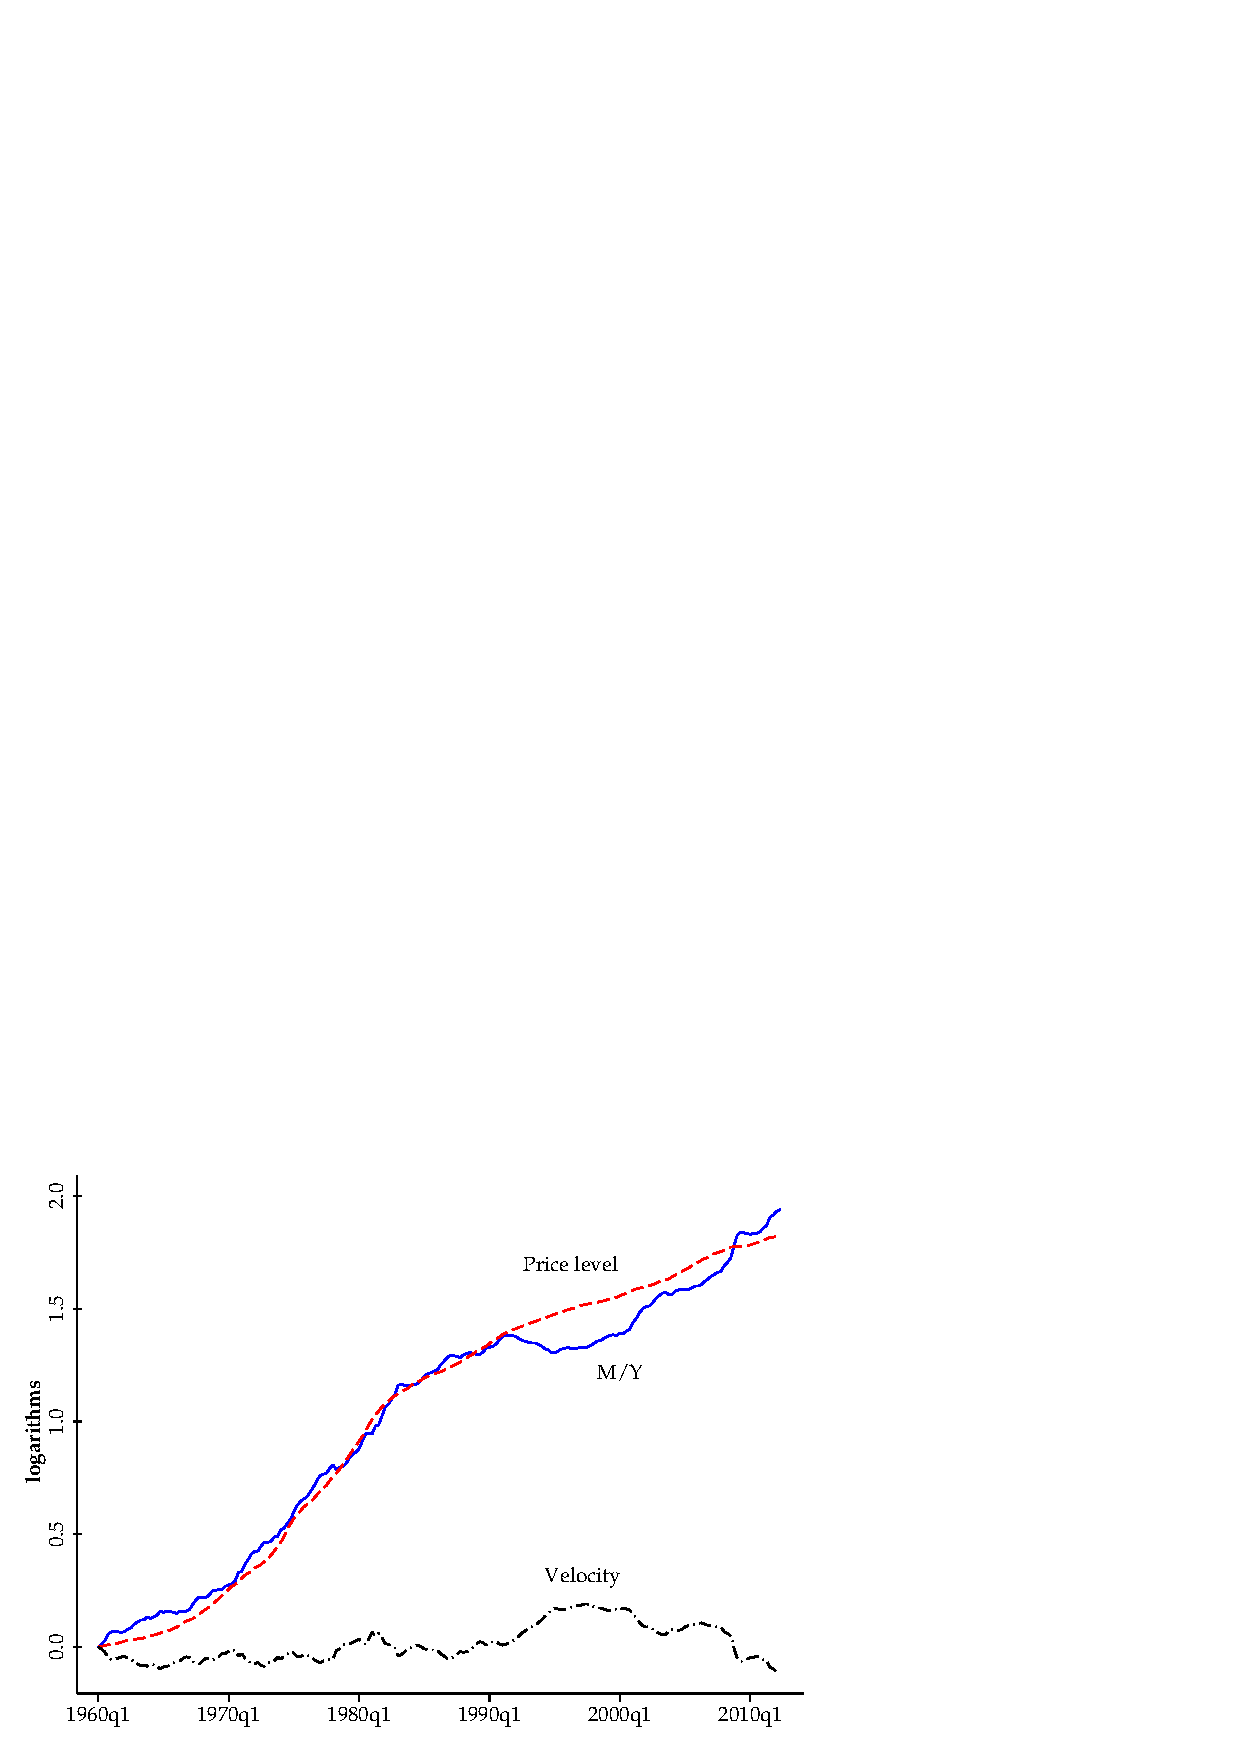
\includegraphics[width=0.8\textwidth]{\figpath Figures/long.pdf}
\end{figure}
%

The evidence for short-run changes is much different.
When we look at year-on-year growth rates,
as we do in Figure~\ref{fig:quantity_short},
velocity has as much short-run volatility as $M/Y$.
As a consequence,
movements in prices are virtually unrelated to movements in money.
To put it bluntly, the quantity theory is a poor guide to short-run fluctuations
in inflation\index{inflation} rates.\index{quantity theory of money|)}

%We'll discuss the short run later in the course, where we try to
%figure out the impact of monetary policy on real output,
%inflation, and interest rates.

\begin{figure}[h]
    \caption{The quantity theory in the short run.}
    \label{fig:quantity_short}
    \centering
    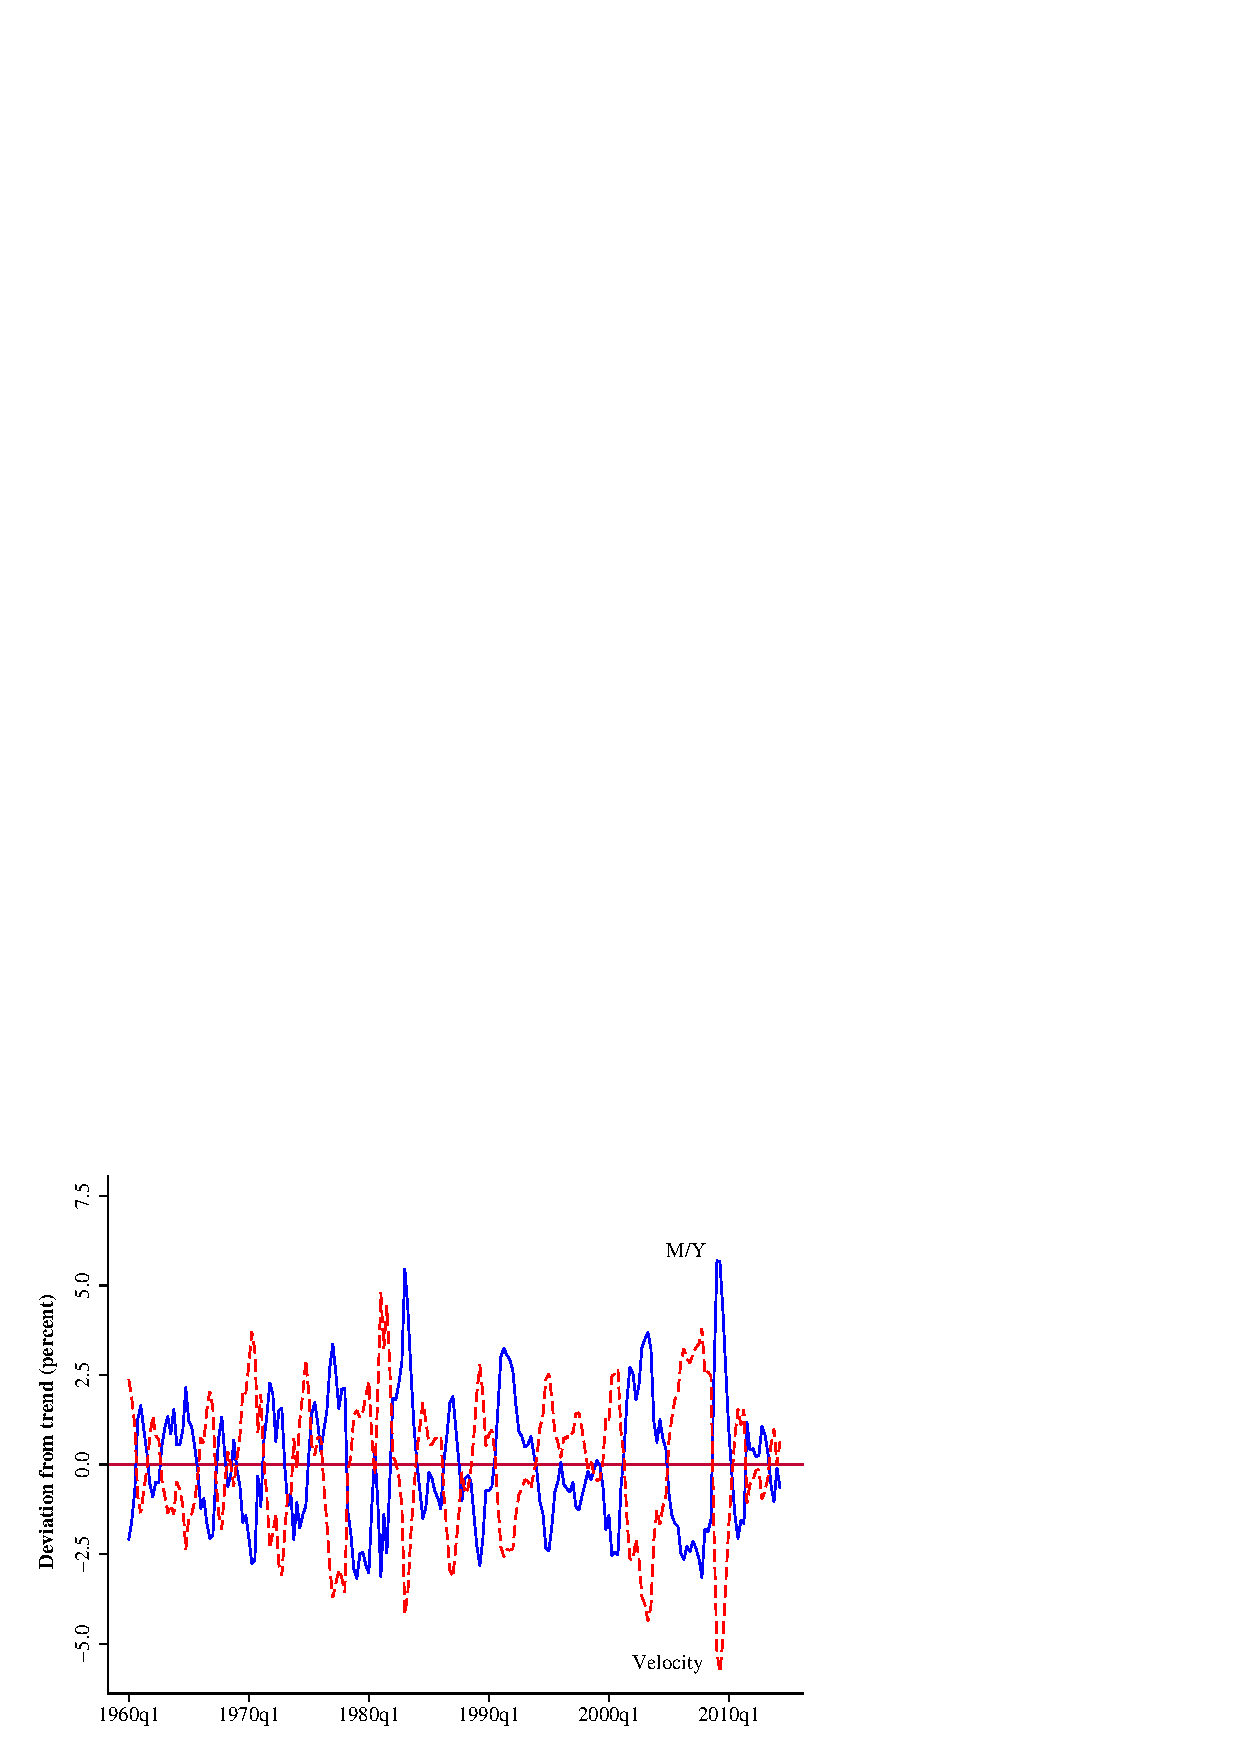
\includegraphics[width=0.8\textwidth]{\figpath Figures/short_1.pdf}
\end{figure}

% ?? change to year-on-year growth rates


\section{Changing the money supply\index{monetary policy!money supply}}

Currency is a liability of the government,
which can (and does) change the quantity in circulation.
To see how this works, it's helpful to take a
step back and consider the broader issue of government debt.
We can divide the government's debt management into two
related pieces.
The first piece is the size of the debt.
Measured in units of currency (dollars, say, or pesos),
the debt changes over time as the government runs surpluses
or deficits.
Mathematically, we might write:
\begin{eqnarray*}
    \mbox{Debt}_{t} &=& \mbox{Debt}_{t-1} + \mbox{Deficit}_t .
\end{eqnarray*}
This is an example of a government budget constraint, something
we'll see more of later on.\index{government budget!budget constraint}
The second piece is the composition of the debt.
In practice, governments have many different liabilities,
but for the purposes of this discussion, let us say, it has two:
government bonds \index{bond} and money (currency).
In both theory and practice,
these two pieces are typically separate,
with the treasury issuing bonds \index{bond} to cover the entire debt
and the monetary authority (central bank \index{central bank|(textbf}) buying back
some of these bonds \index{bond} and issuing money in return.

Day-to-day monetary policy in most countries consists of what we term
{\it open-market operations\/}:  purchases or sales of
government debt (bonds\index{bond}).
At any point in time, the treasury's balance sheet looks
something like:
%\begin{center}
%\begin{tabular}{lr|lr}
%\multicolumn{4}{l}{Central bank \index{central bank}} \\
%\hline
%Assets\phantom{ities} &\phantom{100}&  Liabilities \\
%\hline
%bonds \index{bond} &  100 & Money & 100
%\end{tabular}
%\end{center}
%
\begin{center}
\begin{tabular}{lr|lr}
\multicolumn{4}{l}{Treasury} \\
\hline
Assets\phantom{ities}  &\phantom{100}&  Liabilities \\
\hline
& & Bonds & 200
\end{tabular}
\end{center}
%
and the central bank's  looks like:
%
\begin{center}
\begin{tabular}{lr|lr}
\multicolumn{4}{l}{Central bank} \\
\hline
Assets\phantom{ities}  &&  Liabilities \\
\hline
Bonds &  100 & Money & 100
\end{tabular}
\end{center}
%
If it seems strange to treat money as a liability of the
central bank (isn't money an asset?),
think of it as a bond \index{bond} with the unusual
feature that its nominal interest rate is zero.
That's what it is, which makes it a good deal for the borrower.\index{interest rate!nominal|(}

An open-market purchase of bonds \index{bond} results in an increase
in bonds \index{bond} held by the central bank and an equal increase in its
monetary liability.
For example, a purchase of 20 worth, of bonds \index{bond} would change its
balance sheet to:
%
\begin{center}
\begin{tabular}{lr|lr}
\multicolumn{4}{l}{Central bank} \\
\hline
Assets\phantom{ities}  &&  Liabilities \\
\hline
Bonds &  120 & Money & 120
\end{tabular}
\end{center}
%
The result is an increase in the amount of money in private hands,
since the private sector (the other side of this transaction)
has reduced its holdings of government bonds \index{bond}
and increased its holdings of money.
Similarly, an open-market sale of bonds \index{bond} would reduce the amount of money in
private hands.

The question we're leading up to is why money growth is so high
in countries with big inflations.
Why does the central bank keep issuing money?


\section{Big Inflations}

If inflation\index{inflation} is as easily cured as Friedman suggests
(``control the money supply''),
why do big inflations happen?
People who live through such
episodes describe them as traumatic; they spend an hour or more
every day converting cash into anything with stable value:  real estate,
cars, foreign assets.
The economy is usually a mess, but whether that is cause or effect is
hard to say.
But if big inflations are so painful, why do governments let them happen?
The problem, typically, starts with a government deficit.\index{government budget!budget deficit@budget (or government) deficit}
A political impasse makes it nearly impossible to reduce the deficit.
Given the government's budget constraint, it must then issue debt.
There is apparently no shortage of ready buyers of US debt
(ditto other developed countries),
but the same can't be said for every country.
If no one will buy its debt,
the only remaining option is to finance the deficit with money
(read: oblige the central bank to purchase bonds\index{bond} from the treasury).
In short, when the government can't
pay its bills in any other way, it pays them with money, which is
easy enough to print.
The effect of this, of course, is inflation.\index{inflation}\index{government budget!budget constraint}

The impact here of fiscal policy (government deficits) on inflation
is referred to as fiscal dominance, because fiscal policy dominates monetary policy.
Nobel Prize-winner Thomas Sargent \index{Sargent, Thomas} and his co-author, Neil Wallace,
described a stark version of this.
They showed that even a central bank that aims for low inflation will fail
if the government issues debt without end.
Think of the problem\index{time consistency} as
a version of the \hyperref[sec:time_cons]{time-consistency problem}\index{time consistency}
discussed in Chapter \ref{chp:insp}.
If everyone knows that the central bank eventually will be compelled to print money
to avoid outright default by the government, inflation expectations
 will rise today despite the central bank's \index{central bank|)} caution. The key is
 that the bank cannot credibly commit to limit future money creation, while
 expectations of the future drive price setting today.

The conventional solution to ending a big inflation\index{inflation} has two parts.  The
first is fiscal discipline: Balance the government budget.  The
second is monetary discipline: Separate the central bank
from the treasury and tell the bank that its job is to maintain
price stability. Though there are many fine points --- how quickly must
the deficit be eliminated?  should the IMF supply short-term
financing?  --- the outlines of the problem and its solution
are clear.\index{government budget!budget deficit@budget (or government) deficit}
%Brazil managed to bring inflation under control by tightening its budget.
Going back to Friedman's quote: Inflation may be a monetary phenomenon,
but the trouble often starts with fiscal policy and the political situation that led to it.
When fiscal imperatives drive monetary policy ---
like the fiscal dominance in the Sargent and Wallace analysis ---
inflation eventually follows.

For someone operating an international business,
the thing to remember is that ``big inflations''
are relatively common.
What do you do if you're hit with one?
You'll probably find that the
most important thing you can do is streamline your cash management.
If you can reduce the payment
terms from (say) 60 days to 30 days, you increase your ``real'' revenue substantially.
You may also find that big inflations\index{inflation} lead to policies --- such as price controls and capital controls   --- that make life more complicated.
Finally, you may find that your financial statements
are highly misleading, since they measure performance in terms of the local
currency, the value of which is changing rapidly.
For a US subsidiary, high inflation triggers a change
in the rules for translating financial entries into dollars for tax and reporting purposes.

\section{Inflation and interest rates}

The interest rates we typically use are nominal: They tell us how much money we get in the future
for a given investment of money today.\index{interest rate|(textbf}
Since inflation\index{inflation} measures the change in the value
of money, it shows up in interest rates.
More concretely, we would say that the nominal interest
rate equals the real interest rate (the interest rate
adjusted for inflation) plus \textit{expected} \index{inflation!expected inflation}
inflation:
\begin{eqnarray}
    i_t &=& r_t + \pi_t^e .
    \label{eq:mpin_fisher}
\end{eqnarray}
For a given real interest rate $r$,
an increase in expected inflation raises the nominal interest rate
one for one.\index{interest rate!real}


Here is the deeper explanation behind equation (\ref{eq:mpin_fisher}).
Consider a one-year interest rate on a Treasury bill. \index{Treasury!Treasury bill}
The rate tells us how many dollars (say)
we get in one year for a given payment of dollars today.
For example, if a 12-month treasury bill has a price
of \$96.15, its annualized yield \index{bond!bond yield}
 is the value of $i$ that solves
%
\begin{eqnarray}
    96.15 &=& \frac{100}{1+i_t}.
    \label{eq:nominal_yield}
\end{eqnarray}
%
In this case, $i_t = 4$ percent.  Thus, each dollar invested today gives us
1.04 dollars in 12 months.
We refer to $i_t$ as the  {\it nominal rate of interest\/} --- nominal because its refers to payments of currency.

For many purposes, we'd like to know not only the dollar yield, but
also how much 1.04 dollars will buy when we get it.  If we expect
the inflation\index{inflation} rate to be 3 percent a year, then we'd guess that three quarters of the
interest will be eaten up by inflation.  The investment gains
us only about one percent in terms of purchasing power.
We refer to the increase in purchasing power as the
{\it real rate of interest\/} --- real because it refers to the
quantity of real consumption it finances.
That gives us equation (\ref{eq:mpin_fisher}).\index{interest rate!real}


We can show this more formally
by translating the words into equations more carefully.
We have just argued that investors are interested not in the money the
bond \index{bond} is a claim to, but in what that money will buy. If by ``what
that money will buy,'' we mean the basket of goods used to construct
the CPI, we can define the real interest rate $r$ as
%
\begin{eqnarray*}
    (96.15/P_t) &=& \frac{100/ P_{t+1}}{1+r_t},
\end{eqnarray*}
%
where $P_{t}$ is the CPI index in year $t$ and $P_{t+1}$ is the
expected value of the same index in year $t+1$. What we are doing
here is expressing the current bond \index{bond} price, measured in terms of what
it will buy, as the discounted value of the principal, also measured
in terms of what it will buy. Doing a little algebra, we find
%
\begin{eqnarray*}
    (1+r_t)(P_{t+1}/P_{t}) &=& 100/96.15.
\end{eqnarray*}
%
Then, equation (\ref{eq:nominal_yield}) tells us that the real and
nominal interest rates are related by
\begin{eqnarray*}
    1 + i_t   &=& (1+r_t)(1+\pi_{t}^e),
\end{eqnarray*}
where $(P_{t+1}-P_t)/P_t $ is the expected inflation rate between
$t$ (now) and $t+1$ (a year from now). Since the product
$r_{t}\pi_{t}^e$ is a small number when expected inflation is low, it follows that
\begin{eqnarray*}
    i_t  &\approx&  r_t + \pi_{t}^e, \ \mbox{for \ small \ values \ of \ $r$ and $\pi_{t}^e$},
\end{eqnarray*}
where $\approx$ means ``equals approximately.''
If we're careful about timing, we see that all three variables
are comparisons between now and one year from now.
Inflation is, therefore, typically understood to be
expected inflation,\index{inflation} since we don't know what inflation
will be when we buy the bond\index{bond}.
In principle, we could also take into account the risk
inherent in inflation --- but we won't.


Now that we're done with definitions, we can ask how inflation
affects nominal interest rates.
In principle, either component (the real rate or expected inflation)
can change the nominal interest rate.
In practice, we typically find that in periods of
high and variable inflation,\index{inflation}
the inflation component dominates.
This is approximately true of the US, where high-inflation periods
(the 1970s and early 1980s)
are high-interest-rate periods, too.
It's even more evident in countries with very high inflation rates.


\section{Velocity reconsidered\index{velocity of money}}

In very-high-inflation environments,
people often find that the inflation\index{inflation} rate accelerates
quickly, often far exceeding the rate of money growth.
One factor here is velocity, which typically
rises sharply with inflation.
Why?
Because inflation (and nominal interest) is effectively a tax on holding money:
The higher the tax, the less money you hold.
During big inflations,
people spend money as soon as they get it, because its
value falls by the minute.
It's common, for example, for people to buy groceries
and gasoline as soon as they get their paychecks;
if they wait even a day or two, their purchasing power falls.

If velocity $V$ rises with inflation\index{inflation}, then we can reconsider
\begin{eqnarray}
    \gamma_M + \gamma_V  &=&  \pi + \gamma_Y .
\end{eqnarray}
If $\gamma_Y$ is approximately constant,
then an increase in money growth not only
produces inflation directly, but
its impact is also magnified by the increase in the
interest rate, which increases velocity ($\gamma_V > 0$).
Similarly, when hyperinflations are reversed,
we often see a larger drop in inflation\index{inflation}
than in money growth, as velocity falls.


\section*{Executive summary}

%\setlength{\leftmargini}{.5\oldleftmargini}
\begin{enumerate}
\item Over long periods of time, inflation is closely related to money growth.

%\item High inflation is usually associated with
%high (nominal) interest rates.

\item Extremely high rates of inflation\index{inflation} are invariably associated with high rates of money growth.

\item High money growth is often the result of financing large fiscal deficits with money.
    The deficits, in turn, often reflect some kind of political gridlock.

\item High inflation is typically associated with high interest rates,
since investors demand higher yields \index{bond!bond yield}
 to compensate for the loss of purchasing
power of the currency.
\end{enumerate}
%\setlength{\leftmargini}{\oldleftmargini}

\section*{Review questions}

%\setlength{\leftmargini}{.5\oldleftmargini}
\begin{enumerate}
\item Policy rule.  Friedman suggested that the Fed might do better to adopt
a rule in which it kept the growth rate of the money supply constant.
\begin{enumerate}
\item If the growth rate of real GDP is 3 percent, on average,
what growth rate of the money supply would deliver
average inflation of 2 percent?
\item What are the strengths and weaknesses of such a policy rule?
\end{enumerate}

Answer.
\begin{enumerate}
\item If velocity is constant, then
equation (\ref{eq:quantity_theory-growth}) gives us
a money growth rate of
\begin{eqnarray*}
    \gamma_M &=& \pi + \gamma_Y
            \;\;=\;\;  2 + 3 \;\;=\;\; 5.
\end{eqnarray*}
In words: Money growth accommodates inflation\index{inflation} and economic growth.
\item Strengths: predictable, good average inflation performance,
avoid major policy mistakes.
Weakness: no room for policy to respond to current conditions.
Compare, for example, policy in the aggregate supply (AS) \index{aggregate supply (AS)}
 and demand model
(coming up).
\end{enumerate}


\item Central bank independence.
Why do many countries make central banks \index{central bank} independent of the treasury?

Answer.  The idea is that monetary policy should focus on good long-term
performance and, to accomplish this, should be immune to
short-term political pressure.
With respect to hyperinflations,
you might argue that if the government does not have access to money finance,
it will be forced to confront its deficit issues earlier,
which is a good thing.



\item Zimbabwe.
Zimbabwe ended its hyperinflation by abandoning its currency.
Even official transactions were switched to either US dollars or
    South African rand.
    Does this seem like a good solution?
    Does it make sense for a country to abandon its currency?

Answer.  There's a long tradition of each country having its own currency,
but there's good reason to think at least some countries would be better
off using someone else's.
Zimbabwe has shown no ability to manage it's own currency effectively,
so using another sounds like a move in the right direction.
There are other examples --- Panama and Ecuador use the US dollar --- and perhaps there should be more.

\item Interest rates and inflation.  Go to
\href{http://research.stlouisfed.org/fred2/}{FRED} and find
the three-month treasury bill rate (TB3MS)
and the consumer price index \index{price index!consumer price index (CPI)}
 (CPIAUCSL).
Manipulate them as needed and graph
the nominal interest rate and inflation rate together.
What do you see?

Answer.  Do it and see!\index{interest rate|)}\index{interest rate!nominal|)}

\end{enumerate}
%\setlength{\leftmargini}{\oldleftmargini}


\section*{If you're looking for more}

%Similar material is covered in most macroeconomics textbooks.
Wikipedia has a nice article on hyperinflation,
including a list of the biggest ones of all time.
%
Steve Hanke and Nicholas Krus survey the compete history of
hyperinflation in
``\href{http://www.cato.org/publications/working-paper/world-hyperinflations}{World Hyperinflations}.''
Search:  ``hanke krus hyperinflation.''
Two really good (but more technical) pieces about specific episodes are
Thomas Sargent,
``\href{http://www.nber.org/chapters/c11452.pdf}{The ends of four big inflations},''
and Thomas Sargent and Joseph Zeira,
``\href{http://www.sciencedirect.com/science/article/pii/S1094202511000147}
{Israel 1983}.''


\section*{Symbols and data used in this chapter}

\begin{table}[H]
\centering
\caption{Symbol table.}
\begin{tabular*}{0.8\textwidth}{l@{\extracolsep{\fill}}l}
\toprule
Symbol & Definition\\
\midrule
$M$            &Money stock\\
$V$            &Velocity of money\\
$P$            &Price level\\
$Y$            &Real output or GDP\\
$\ln$        &Natural log\\
$\gamma_x$    &Continuously compounded growth rate of $x$\\
$\pi$         &Inflation ($= P$)\\
$\pi^{e}$    &Expected Inflation\\
$i$            &Nominal interest rate\\
$r$            &Real interest rate ($= i- \pi^e$)\\
\bottomrule
\end{tabular*}
\end{table}

\begin{table}[t]
\centering
\caption{Data table.}
\begin{tabular*}{0.8\textwidth}{l@{\extracolsep{\fill}}l}
\toprule
Variable & Source\\
\midrule
Nominal GDP                    &GDP\\
M2 monetary aggregate        &M2SL\\
M2 velocity                    &M2V\\
Consumer price index
        &CPIAUCSL\\
\bottomrule
\addlinespace
\end{tabular*}
\begin{minipage}{0.8\textwidth}
\footnotesize{To retrieve the data online, add the identifier from the source column to \url{http://research.stlouisfed.org/fred2/series/}.  For example, to retrieve nominal GDP, point your browser to \url{http://research.stlouisfed.org/fred2/series/GDP}}
\end{minipage}
\end{table}

%%%%%%%%%%%%%%%%%%%%%%%%%%%%%%%%%This could cause problems later!%%%%%%%%%%%%%%%%%%%%%%%%%%%%%%%%%%%%%%%%
%%KR: the last table ends up on its own page, but vertically centered.  To force the table to the top, I've
%%added these two aweful lines below.
\vfill
\phantom{x}
%%%%%%%%%%%%%%%%%%%%%%%%%%%%%%%%%%%%%%%%%%%%%%%%%%%%%%%%%%%%%%%%%%%%%%%%%%%%%%%%%%%%%%%%%%%%%%%%%%%%%%%%% 
\include{notes_asad}
\chapter{Policy in the AS/AD model \index{AS/AD model}
}\label{chp:pasad}
\hypertarget{asadpolicy}{}

\input{\blurbpath Blurbs/blurbs_asadpolicy}
\rule{\textwidth}{1pt}

We've seen that aggregate demand
 and supply can shift on their own or,
sometimes, as a result of changes in policy,
including monetary policy.
But what policy changes are called for?
Should we always shift the aggregate demand
 curve to maintain
low inflation?\index{inflation}  High output?
Are these two objectives in conflict?
The short answer is that we should respond differently to changes in supply and demand.
A somewhat longer answer follows.


\section{Objectives of policy}

The traditional guide to economic policy is the invisible hand.
If markets work well, then we simply leave them to do their job.
If not, we may act to facilitate their operation.
In the aggregate demand\index{aggregate demand (AD)}
 and supply framework,
the idea is that the   long-run aggregate supply \index{aggregate supply (AS)!long-run aggregate supply}\index{aggregate supply (AS)}
 curve is where the uninhibited operation of markets would lead us.
In the short run, sticky wages (or other market imperfections)
may delay the adjustment, but that's
where the invisible hand ultimately would direct us.
One consequence is that there's no
compelling reason to change aggregate demand \index{aggregate demand (AD)}
to increase output beyond its long-run equilibrium value.
We might be able to do it, but it won't make us better off.
In a sense, we will have tricked people into working more than they
want, typically by reducing their real wages through unexpected inflation.\index{inflation}

The first objective of policy, then,
is to get output as near as possible to
the level associated with the long-run
aggregate supply\index{aggregate supply (AS)}
 curve AS$^*$.
This is important enough a concept that people have given it
lots of names:  potential output, full employment output, and so on.
We'll call it {\it potential output\index{potential output}\/}, with the understanding that it's
the long-run equilibrium, not an upper bound.
The {\it output gap \index{output gap}\/} is a related concept:
the difference between actual and potential output.
In practice, potential output is a little slippery,
because the   long-run aggregate supply \index{aggregate supply (AS)!long-run aggregate supply}\index{aggregate supply (AS)}
 curve isn't something we observe.
We have a variety of ways of estimating potential output,
ranging from the complex  to
the pragmatic (a smooth trend line drawn through actual output).
We give some examples (and links) at the end of the chapter.

The second objective of policy is price stability.
That's not an obvious implication of the invisible hand,
but experience has taught us that low and (especially) stable rates of
inflation\index{inflation} are associated with good macroeconomic performance.
You might ask whether we'd be better off with no inflation,
low inflation (say, two or three percent a year),
or even modest deflation (yes, there are theoretical arguments
for that).
However, experience suggests that it doesn't matter too much. Any stable target is better than
the high and variable inflation that the US and many other countries
experienced in the 1970s.


%%%%%%%%%%%%%%%%%%%%%%%%%%%%%%%%%%%%%%%%%%%%%%%%%%%%%%%%%%%%%%%%%%%%%%%%%%%%
%  Supply and demand diagram
\begin{figure}[!ht]
\caption{The impact of an adverse demand shock.}
    \label{fig:asad-m}
%
\centering
\setlength{\unitlength}{0.075em}
\begin{picture}(250,200)(0,0)
%\footnotesize
\thicklines

% horizontal axis
\put(-30,0){\vector(1,0){300}}
\put(255,-16){$Y$}
\put(142,-16){$Y^*$}

% vertical axis
\put(0,-20){\vector(0,1){200}}
\put(-15,155){$P$}

% demand
\put(25,165){\line(4,-3){200}}\put(230,10){AD$'$}
\put(65,165){\line(4,-3){200}}\put(270,10){AD}

% supply
\put(25,13){\line(4,3){200}} \put(230,160){AS}
%\put(65,13){\line(4,3){200}} \put(270,160){AS$'$}
\put(146.4,0){\line(0,1){170}} \put(138,175){AS$^*$}

% equilibrium labels
\put(105,85){\footnotesize B}
\put(150,115){\footnotesize A}
%\put(138,64){\footnotesize C}
% dotted lines
%\qbezier[31]{(133,0)(133,46)(133,92)}
%\qbezier[45]{(0,92)(67,92)(133,92)}
%\qbezier[45]{(0,72)(67,72)(133,72)}

\end{picture}
\begin{minipage}{0.7\textwidth}
\vspace{0.45in}
{\footnotesize Aggregate demand\index{aggregate demand (AD)}
 AD shifts left to AD$'$, moving the short-run equilibrium from A to B.}
\end{minipage}

\end{figure}
%%%%%%%%%%%%%%%%%%%%%%%%%%%%%%%%%%%%%%%%%%%%%%%%%%%%%%%%%%%%%%%%%%%%%%%%%%%%



\section{Policy responses to supply and demand shocks}

With potential output and stable prices as our objectives,
how should policy respond to changes in aggregate supply\index{aggregate supply (AS)}
 or demand?
Curiously, the answer depends on whether we face supply shocks or demand
shocks.

How should we respond to demand shocks?
Consider a negative demand shock,
illustrated by Figure \ref{fig:asad-m}.
The long-run equilibrium is point A,
where aggregate supply\index{aggregate supply (AS)}
 AS$^*$ and aggregate demand\index{aggregate demand (AD)}
 AD cross.
Suppose that consumer pessimism shifts the aggregate demand\index{aggregate demand (AD)}
 curve to AD$'$, leaving us at point B.
What should we do?
If we do nothing, we fail on both of our objectives because output is below potential and prices have fallen.
The appropriate policy, then, is to shift the demand curve
back to AD, perhaps by expanding the money supply.

That's a general rule:  Policy should offset demand shocks.
In this case, there is no conflict between our two goals
of hitting potential output and maintaining stable prices.
The policy lesson:  We should resist or offset demand shocks.


%%%%%%%%%%%%%%%%%%%%%%%%%%%%%%%%%%%%%%%%%%%%%%%%%%%%%%%%%%%%%%%%%%%%%%%%%%%%
%  Supply and demand diagram
\begin{figure}[!ht]
\caption{The impact of an increase in the price of oil.}
\label{fig:asad-oil}
%
\centering
\setlength{\unitlength}{0.075em}
\begin{picture}(250,200)(0,0)
%\footnotesize
\thicklines

% horizontal axis
\put(-30,0){\vector(1,0){300}}
\put(255,-16){$Y$}
\put(142,-16){$Y^*$}
\put(102,-16){$Y^{*\prime}$}

% vertical axis
\put(0,-20){\vector(0,1){200}}
\put(-15,155){$P$}

% demand
\put(25,165){\line(4,-3){200}}\put(230,10){AD}
%\put(65,165){\line(4,-3){200}}\put(270,10){AD$'$}

% supply
\put(65,13){\line(4,3){200}} \put(270,160){AS}
\put(25,13){\line(4,3){200}} \put(230,160){AS$'$}
\put(146.4,0){\line(0,1){170}} \put(138,175){AS$^*$}
\put(106.4,0){\line(0,1){170}} \put(98,175){AS$^{*\prime}$}

% equilibrium labels
\put(150,55){\footnotesize A}
\put(122,75){\footnotesize B}
\put(95,94){\footnotesize C}
\put(95,76){\footnotesize D}
%\put(95,54){\footnotesize D}
% dotted lines
%\qbezier[31]{(133,0)(133,46)(133,92)}
%\qbezier[45]{(0,92)(67,92)(133,92)}
%\qbezier[45]{(0,72)(67,72)(133,72)}

\end{picture}
\begin{minipage}{0.7\textwidth}
\vspace{0.45in}
{\footnotesize Aggregate supply\index{aggregate supply (AS)}
 curves shift left from AS/AS$^*$ to AS$'$/AS$^{*\prime}$,
moving the short-run equilibrium from A to B.}
\end{minipage}

\end{figure}
%%%%%%%%%%%%%%%%%%%%%%%%%%%%%%%%%%%%%%%%%%%%%%%%%%%%%%%%%%%%%%%%%%%%%%%%%%%%


How should we respond to supply shocks? \index{supply shocks}
Consider the situation depicted in Figure \ref{fig:asad-oil}:
an adverse supply shock that moves us from A to B.
Should policy try to offset the decline in output?
If we follow our logic, the answer is no;
we want to move output as close to the long-run aggregate supply \index{aggregate supply (AS)!long-run aggregate supply}\index{aggregate supply (AS)}
curve AS$^{*\prime}$ as possible.
We do this by moving the aggregate demand\index{aggregate demand (AD)}
 curve left (left!) until it intersects
both aggregate supply\index{aggregate supply (AS)}
 curves at point D.
At this point, the price level is the same as it was at A,
so we have delivered stable prices.
Output has fallen more than if we had not acted,
but that's what the invisible hand suggests.
The policy lesson:  We should acquiesce to or accommodate
supply shocks.

The basic lesson, then, is that we want to react differently to
changes in output that result from supply and demand shocks.
We should resist demand shocks and accommodate supply shocks.
The difficulty, in practice, is knowing which is which.
If we guess wrong, we can make things worse, perhaps a lot worse.

By some interpretations, the Fed made exactly this mistake in the 1970s.
With output falling and inflation rising, the Fed increased the money
supply to keep output up.
With hindsight, the OPEC oil price increase is understood to be an
adverse supply shock.
It reduced output, but there was little we could do about it.
When we increased the money supply, the consequence was that low
output was accompanied by even higher inflation\index{inflation} than before.
Having failed to understand the problem,
we decided to give it a name:  stagflation.


\section*{Executive summary}

%\setlength{\leftmargini}{.5\oldleftmargini}
\begin{enumerate}
\item We typically think of the goals of macroeconomic
policy as keeping inflation low and output near the long-run
supply curve.

\item As a general rule, policy should resist changes in output
triggered by shifts in demand and accommodate/acquiesce
to changes triggered by shifts in supply.
\end{enumerate}
%\setlength{\leftmargini}{\oldleftmargini}

%\begin{comment}
\section*{Review questions}

%\setlength{\leftmargini}{.5\oldleftmargini}
\begin{enumerate}
\item Consider the situation in Figure \ref{fig:asad-m},
where an adverse demand shock moves us from A to B.
\begin{enumerate}
\item What is your welfare analysis of the change?
In what ways is B better than A?  Worse?
\item How would your answer change if AD shifted to the right,
rather than the left?
\end{enumerate}

Answer.
\begin{enumerate}
\item Recall the objectives of policy:  (i)~stable prices
and (ii)~output at its long-run equilibrium value $Y^*$.
In this case prices fall, so we fail on (i), and output moves
away from $Y^*$, so we fail on (ii).
\item In this case output and prices both rise,
but both are bad from a welfare point of view.
Note specifically that it's not true that more output is better.
\end{enumerate}

\item Current economic conditions.
\begin{enumerate}
\item What have inflation\index{inflation} and GDP growth been over the past year?
\item Would you say demand has shifted or supply relative to the year before?
\item Using this information and anything else you think is appropriate,
where is the economy relative to the long-run equilibrium level of output $Y^*$?
\end{enumerate}

Answer.
\begin{enumerate}
\item [(a,b)] The idea is to look at the numbers and decide whether
we seem to be experiencing a shift in supply or demand --- or perhaps neither.
If inflation and output growth have moved together, we'd say demand.
If they've moved in opposite directions, we'd say supply.

\item[(c)] Good question.  What would you suggest?
\end{enumerate}

\item Stimulus in China.
In 2009, China responded to the financial crisis by
implementing a massive program of government spending
on infrastructure.
Your mission is to outline the argument for or against such a program
using the aggregate supply\index{aggregate supply (AS)}
 and demand (AS/AD) framework.
%
\begin{enumerate}

\item Over the last year, output growth and inflation\index{inflation} have both fallen in China.  Would you say this comes from a shift in supply or demand?
    Illustrate your answer with the appropriate diagram.

\item Describe the impact of
a large increase in government spending on infrastructure projects.
What is the likely impact on output?  On inflation?

\item What are the traditional goals of macroeconomic policy,
expressed in terms of aggregate supply\index{aggregate supply (AS)}
 and demand?
Does the Chinese spending program move them closer to these goals?
\end{enumerate}

Answer.
\begin{enumerate}
\item Shifts in demand move output and prices in the same direction,
shifts in supply move them in opposite directions.
(By longstanding tradition, we interpret output as output growth
and prices and inflation.)
Since they both fell, we would interpret this as a shift left in demand.

\item This is a {\it purchase\/} of goods; therefore, it affects demand.
A shift right in demand increases both output growth and inflation.

\item The goals are (i) output equal to the   long-run aggregate supply \index{aggregate supply (AS)!long-run aggregate supply}\index{aggregate supply (AS)}
 curve AS$^*$ and (ii)~stable prices.
    The answer depends where you start:  Are we to the left of AS$^*$ prior to the stimulus?  If so, then the stimulus program moves
output in the right direction.
Ditto with inflation:\index{inflation}  If we start with stable prices,
the stimulus generates inflation.
\end{enumerate}

\item {Aggregate implications of employer-provided health insurance.}
By an accident of history, health insurance in the US is generally
provided by employers.
Suppose a sharp rise in healthcare costs leads firms to hire fewer workers.
\begin{enumerate}
\item How would you represent this in an aggregate supply\index{aggregate supply (AS)}
 and demand diagram?
Which curve shifts?  In which direction?
\item What is the new short-run equilibrium?  Long-run equilibrium?
What happens to inflation and output?
\item How should the central bank \index{central bank} respond?
Be specific about its goals and how it would accomplish them.
\end{enumerate}


Answer.
\begin{enumerate}
\item Since we're talking about firms and production,
this must involve the supply side of the model.
We shift AS and AS$^*$ to the left, both by the same amount.
See the figure below.

\item We started at A.
After the shift, we move to a new short-run equilibrium at B,
where the new AS crosses AD.
Evidently output falls and prices rise.

Eventually we move to a new long-run equilibrium at C,
where AD crosses the new AS$^*$.
At this point, output has fallen more and prices have risen more.

\begin{center}
\begin{figure*}[t]
\centering
\setlength{\unitlength}{0.075em}
\begin{picture}(300,200)(-10,-10)
%\footnotesize
\thicklines

% horizontal axis
\put(-30,0){\vector(1,0){300}}
\put(255,-16){$Y$}
\put(142,-16){$Y^*$}
\put(102,-16){$Y^{*\prime}$}

% vertical axis
\put(0,-20){\vector(0,1){200}}
\put(-15,155){$P$}

% demand
\put(25,165){\line(4,-3){200}}\put(230,10){AD}
%\put(65,165){\line(4,-3){200}}\put(270,10){AD$'$}

% supply
\put(65,13){\line(4,3){200}} \put(270,160){AS}
\put(25,13){\line(4,3){200}} \put(230,160){AS$'$}
\put(146.4,0){\line(0,1){170}} \put(138,175){AS$^*$}
\put(106.4,0){\line(0,1){170}} \put(98,175){AS$^{*\prime}$}

% equilibrium labels
\put(150,55){\footnotesize A}
\put(122,75){\footnotesize B}
\put(95,94){\footnotesize C}
\put(95,76){\footnotesize D}
%\put(95,54){\footnotesize D}
% dotted lines
%\qbezier[31]{(133,0)(133,46)(133,92)}
%\qbezier[45]{(0,92)(67,92)(133,92)}
%\qbezier[45]{(0,72)(67,72)(133,72)}

\end{picture}
\end{figure*}
\end{center}


\item The central bank \index{central bank} has two goals:  stable prices and output
at its long-run equilibrium.
Here we've moved from A to C.
We're ok at C on the second goal:  output fell,
but that's the long-run equilibrium so there's nothing monetary policy
can do about that.
(We could consider other policies, but they're not the job of the central bank.\index{central bank})

Where C is bad is with respect to price stability:  prices are higher.
So the central bank \index{central bank} could shift AD to the left, giving us the same
long-run output but lower prices.
The central bank \index{central bank} would accomplish this by reducing the money supply,
which it might do by targeting a higher interest rate.
\end{enumerate}

% =============================================================================
\item The supply and demand of Abenomics.
Shinzo Abe was elected Prime Minister of Japan in December 2012
after two decades of slow growth and falling prices.
He pledged dramatic policy changes to revive the Japanese economy,
dubbed the ``three arrows'' of ``Abenomics.''
We consult the Economist Intelligence Unit for specifics:
%
\begin{itemize}
\item Fiscal stimulus.  A sizeable economic stimulus package was passed by parliament in
February 2013, and a smaller one in October.
This is expected to produce a budget deficit of 8\% in 2013.
\item Monetary stimulus. A plan to double Japan's
money supply within two years was implemented in April 2013 to help to achieve the Bank of Japan's
target of 2\%  inflation.
\item Structural reform.
This is less clearly articulated, but some observers hope for a range of micro-based reforms,
including loosening product-market regulations that reduce productivity,
tightening corporate requirements for funding pensions,
creating a more flexible labor market,
and reducing subsidies to an inefficient agricultural sector.
\end{itemize}
%
Your mission is to explore the impact of the three arrows using the aggregate supply and demand
framework.
\begin{enumerate}
\item Explain, for each ``arrow,'' whether it affects supply or demand.
Which way does each one shift the appropriate curve(s)?
\item Compare the short- and long-term impact on output of the three policies.
Which are likely to have the greatest impact in the short term?
In the long term?
\end{enumerate}

\needspace{4\baselineskip}
Answer.
\begin{enumerate}
\item We have:
\begin{itemize}
\item Fiscal stimulus. This shifts aggregate demand to the right.
\item Monetary stimulus. Same.
\item Structural reform. This shifts both aggregate supply curves to the right.
\end{itemize}

\item Fiscal and monetary stimulus raise output in the short run.
They have no long-run impact on output.

Structural reform is likely the most important of the arrows
for the long-term performance of the Japanese economy.
It should raise output long term, in large part by increasing productivity,
but short-term transition issues could go the other way.
It's also the arrow that's been executed least aggressively.
\end{enumerate}


%\begin{figure}[h]
%    \centering
%    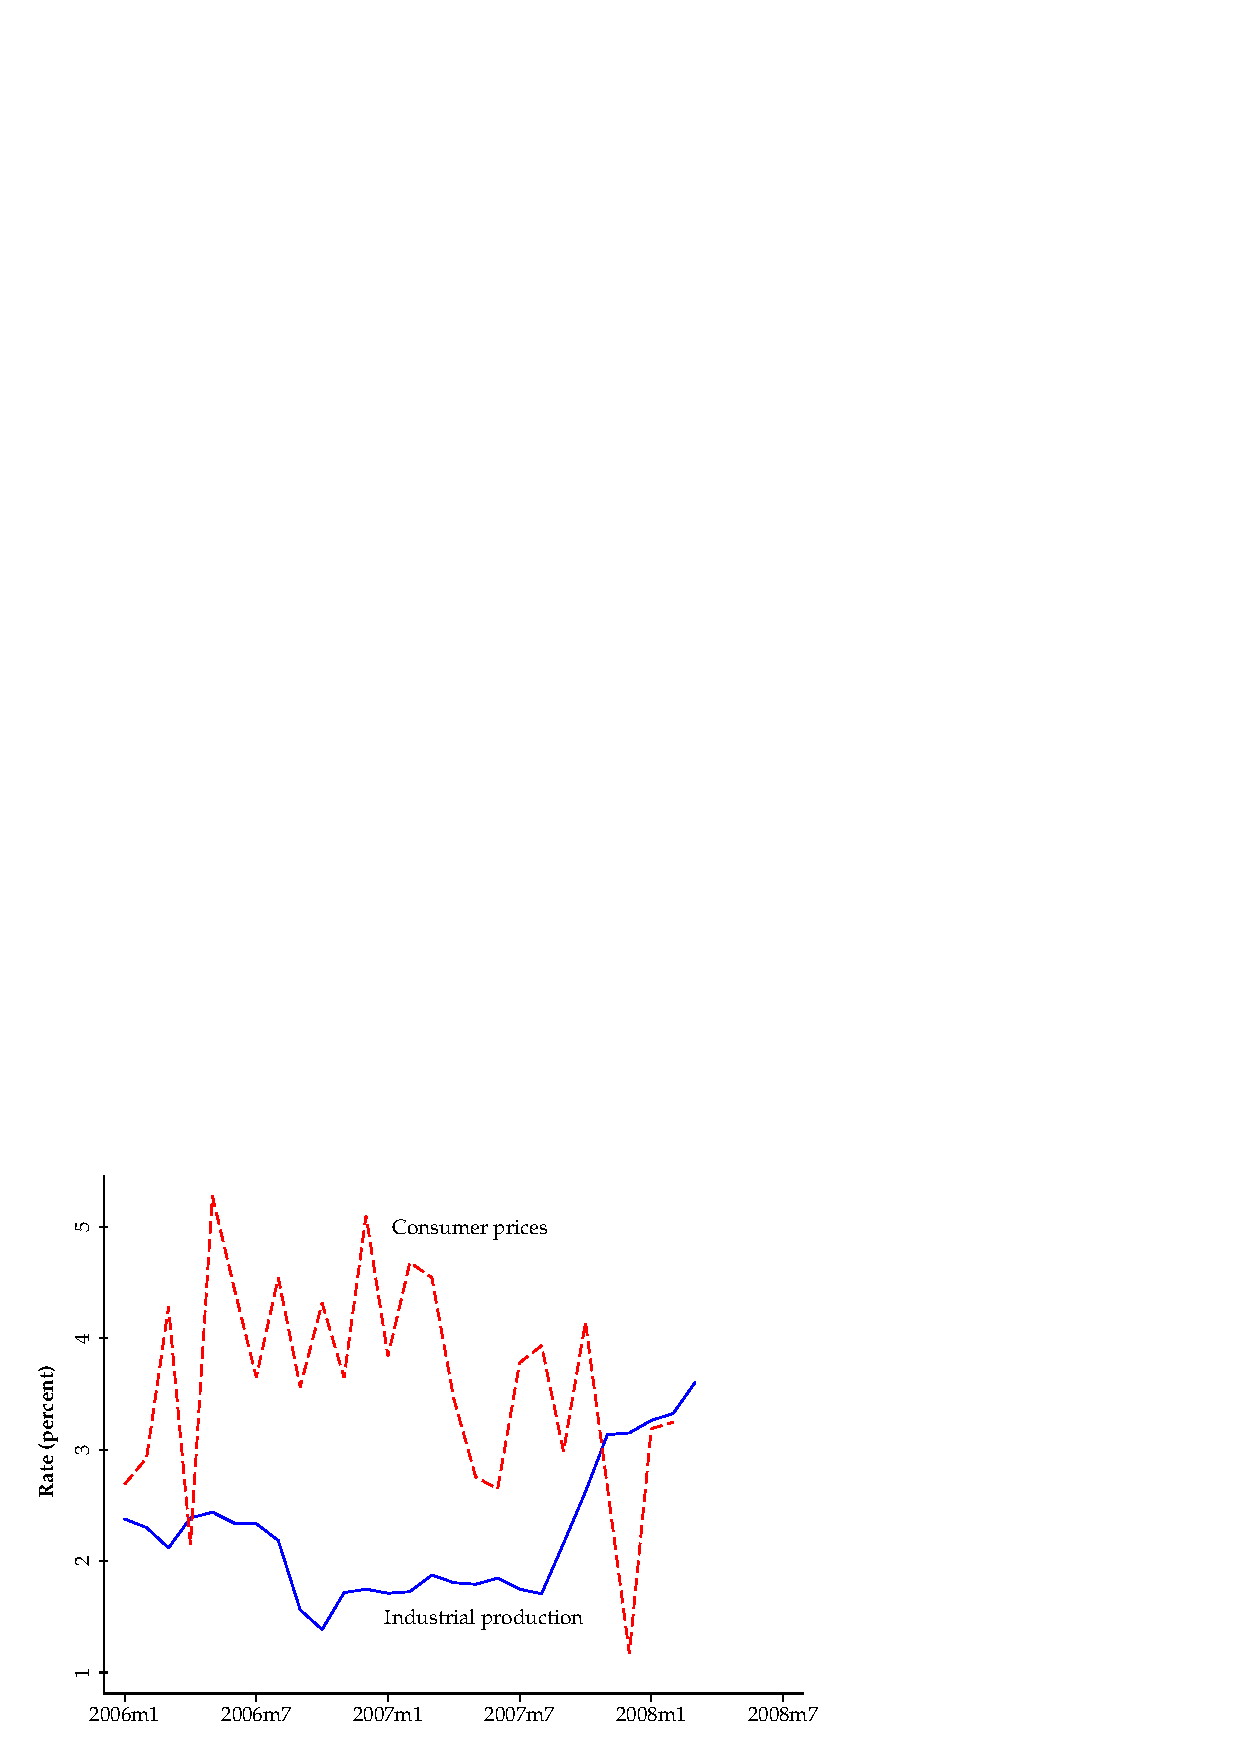
\includegraphics[width=0.8\textwidth]{Figures/eu_asad.pdf}
%    \caption{Growth in prices and industrial production in the
%    Euro Zone.}
%    \label{fig:ez}
%\end{figure}
%
%\item aggregate supply (AS) \index{aggregate supply (AS)}
% and demand in the Euro Zone,
%May 2008.
%As the CFO of Heineken International, you are considering
%the likely evolution of interest rates in the Euro Zone.
%You quickly run through the following questions:
%%
%\begin{enumerate}
%
%\item Over the 2-year period as a whole,
%    what has happened to inflation and output?
%    See Figure \ref{fig:ez}.
%
%\item In the aggregate supply (AS) \index{aggregate supply (AS)}
% and demand framework,
%    do you think the movements in prices and output
%    you mentioned above suggest a shift in supply or demand?  Why?
%    In principle,
%    how should the European central bank \index{central bank} respond to such a shift?
%
%\item How do you think the European central bank \index{central bank} is
%likely to respond?
%How do you see short-term Euro Zone
%interest rates moving over the next 12 months? Why?
%
%\end{enumerate}
%
%
%%\begin{comment}
%Answer.
%\begin{enumerate}
%\item Inflation is up sharply, output is flat to down.
%
%\item The combination in (a) suggests a shift up/left in supply.
%Why?  Because output and inflation have moved in opposite directions.
%Since supply shocks should be accommodated/reinforced,
%the ECB should raise the short-term interest rate.
%
%\item The ECB's primary mission is stable prices,
%so you should see an increase in interest rates.
%This could also be expressed in terms of a Taylor rule,
%possibly with a larger coefficient on inflation
%than output growth.
%\end{enumerate}
\end{enumerate}
%\setlength{\leftmargini}{\oldleftmargini}


\section*{If you're looking for more}

The measurement of potential output has generated some interesting debate.
The bottom line, in our view, is that there's usually some question
where the   long-run aggregate supply \index{aggregate supply (AS)!long-run aggregate supply}\index{aggregate supply (AS)}
 curve is. Here is a range of opinion on the subject:
%
\begin{itemize}
\item The Congressional Budget Office (CBO) reviews a number of approaches.
Search: ``cbo potential output.''
%\url{http://www.cbo.gov/sites/default/files/cbofiles/ftpdocs/51xx/doc5191/03-16-gdp.pdf}.

\item Former Fed Governor Frederic Mishkin's speech,
``Estimating potential output,'' is another good overview.
Search:  ``mishkin potential output.''

\item The Kansas City Fed's 2005 Jackson Hole Symposium has
an interesting exchange between Robert Hall and Greg Mankiw.
Hall argues that potential output may very well not be smooth,
which would contradict most measures of it.
As a practical matter, this would change our view of monetary policy dramatically
since many of the movements we see in GDP would be the result of the invisible hand
and, therefore, not something for policymakers to resist.
Mankiw says maybe, maybe not.
Search:  ``Jackson Hole Symposium 2005.''
%\centerline{\url{http://www.kc.frb.org/publications/research/escp/escp-2005.cfm}}
\end{itemize}

\needspace{18\baselineskip}
\section*{Symbols and data used in this chapter}

\begin{table}[H]
\centering
\caption{Symbol table.}
\begin{tabular*}{0.7\textwidth}{l@{\extracolsep{\fill}}l}
\toprule
Symbol & Definition\\
\midrule
$Y$    &Real output (=real GDP)\\
$Y^*$    &Equilibrium (or potential) output\\
${Y^{*}}'$    &New equilibrium (or potential) output\\
AS    &Short-run aggregate supply \\
AS$^*$    &  Long-run aggregate supply\\
AD    &Aggregate demand\\
AD$'$    &Aggregate demand after a shock\\
AS$'$    &Aggregate supply  after a shock\\
\bottomrule
\end{tabular*}
\end{table}

\begin{table}[h]
\centering
\caption{Data table.}
\begin{tabular*}{0.7\textwidth}{l@{\extracolsep{\fill}}l}
\toprule
Variable & Source\\
\midrule
NBER recession indicator    &USRECM\\
CBO real potential GDP        &GDPPOT\\
Oil Price (WTI)                &OILPRICE\\
\bottomrule
\addlinespace
\end{tabular*}
\begin{minipage}{0.7\textwidth}
\footnotesize{To retrieve the data online, add the identifier from the source column to \url{http://research.stlouisfed.org/fred2/series/}.
For example, to retrieve oil prices, point your browser to
\url{http://research.stlouisfed.org/fred2/series/OILPRICE}}
\end{minipage}
\end{table}

\include{notes_monpol}

% Other topics
\part{Crises and Other Topics}


\chapter*{Crisis Overview}
\hypertarget{}{}

\rule{\textwidth}{1pt}

This outline covers key concepts from the third part of the course:
macroeconomic crises and other topics.
It is not exhaustive, but is meant to help you
(i)~anticipate what is coming and
(ii)~organize your thoughts later on.

\medskip
\textbf{\hyperref[chp:tax]{\underline{Taxes}} and \hyperref[chp:dbdf]{\underline{Government Debt and Deficits}}}

\textbf{Tools:} Welfare triangles; government budget constraint; debt dynamics.

\textbf{Key Words:} Tax wedge; deadweight loss; primary deficit/surplus.

\textbf{Big Ideas:}
\vspace{-0.1in}
\begin{itemize}
\item Tax systems should be (i) administratively simple and transparent and (ii) have a broad tax base. 
\item Government spending must be paid for, either now through taxes, or in the
future by running primary surpluses.
\item Changes in the ratio of debt to GDP have three sources:
interest, growth, and primary deficits.
\end{itemize}


\begin{comment}
\hyperref[chp:bop]{\textbf{\underline{Balance of Payments}}}

\textbf{Tools:} Sustainability analysis.

\textbf{Key Words:} Current account; net exports; capital account; net foreign assets.

\textbf{Big Ideas:}
\vspace{-0.1in}
\begin{itemize}
\item Current account deficits imply that the country is borrowing from the rest of the
world; current account surpluses mean that the country is lending to the rest of the
world.
\item Balance of payment deficits are unsustainable when net foreign liabilities grow faster than the economy as a whole.
\end{itemize}
\end{comment}


\textbf{\hyperref[chp:fxf]{\underline{Exchange-Rate Fluctuations}} and \hyperref[chp:fxr]{\underline{Exchange-Rate Regimes}}}

\textbf{Tools:} Arbitrage arguments; central bank balance sheet.

\textbf{Key Words:} Real and nominal exchange rates; purchasing power parity; covered/uncovered interest parity; 
spot and forward exchange rates; the carry trade; convertibility; capital mobility; capital controls; fixed (pegged) vs. flexible (floating) exchange rate regimes; foreign exchange reserves; sterilization; speculative attack.

\needspace{4\baselineskip}
\textbf{Big Ideas:}
\vspace{-0.1in}
\begin{itemize}
\item Short-run movements in real exchange rates are largely unpredictable.  
\item Countries adopt different exchange rate regimes:  fixed, floating, and in between. 
The trilemma limits our policy options:  we can choose only two of
(i)~fixed exchange rate, (ii)~free flow of capital,
and (iii)~discretionary monetary policy.
\item Fixed exchange rate regimes must be defended through open market operations and are vulnerable to speculative attack.
\end{itemize}

\textbf{\hyperref[chp:cris]{\underline{Macroeconomic Crises}}}

\textbf{Tools:} Crisis triggers and indicators.

\textbf{Key Words:} Sovereign default; bank runs and panics; refinancing (rollover) risk; leverage; conditionality;
solvency and liquidity.

\textbf{Big Ideas:}
\vspace{-0.1in}
\begin{itemize}
\item Common triggers of macroeconomic crises are sovereign debt problems, financial fragility,
and fixed exchange rates.

\item Measures related to these triggers can help identify countries in trouble:
debt and deficits, financial weakness, exchange rate regime, and so on.

\item The goals of crisis prevention and crisis management are often at odds.
\end{itemize}

\include{notes_taxes}
\include{notes_deficits}
\include{notes_bop}
\include{notes_fx}
\include{notes_fxregimes}
\chapter{Macroeconomic Crises}\label{chp:cris}
\hypertarget{crises}{}

\input{\blurbpath Blurbs/blurbs_crises}
\rule{\textwidth}{1pt}

Economies periodically experience {\it crises\/}:
economic downturns that are not only larger than typical recessions
but qualitatively different.
The idea is now fresh in our minds,
but similar episodes have occurred throughout recorded history.
They're less common in modern, developed countries,
but they can happen anywhere.
Like snowflakes and business cycles, no two are exactly the same,
but they share some common features.


\section{Classic crisis triggers }

There are three classic triggers of macroeconomic crises:
sovereign debt, financial fragility, and a fixed exchange rate.\index{exchange rate regime!fixed exchange rate}

\textbf{Sovereign debt problems.\index{government debt!sovereign debt}}
If investors fear that a government may not repay its debt,
the market for debt collapses, often taking the economy with it.
In the old days, wars were the standard problem.
Wars are expensive, and if investors thought the expense was more
than the government was willing or able to bear,
they would stop buying the debt.
In modern times, governments spend money on many things besides wars,
but the possibility of default remains.
Argentina in 2002 and Greece today are recent examples.
These experiences remind us that sovereign debt need not be risk-free.

The central issue with government debts is sovereignty.
If a corporation defaults, the creditors take it to court
and claim the assets.
With governments, there's no such mechanism, and the process
is sloppier as a result.

\textbf{Financial fragility.}
We know from centuries of experience that when the
financial system freezes up,
economic activity slows down sharply.
We saw that in 2008,
but the same thing happened during the Bank of England Panic of 1825,
the Baring Crisis of 1890,
the US Panic of 1907,
Japan and Scandinavia in the 1990s,
and many other occasions.
It's a feature of even advanced financial systems that they
sometimes break.

In most cases, these financial problems follow from
poor investments (real estate is a common example),
which put the solvency of financial institutions in question.
The problems tend to snowball: Worries about the viability of one firm may lead others to
reduce their lending, leading to a cycle of retrenchment
that puts even sound firms in trouble.
The word ``panic'' is apt here and stems
from the imperfect information that investors have
when deciding where to put their money.


\textbf{Fixed exchange rates.} For whatever reason, fixed exchange rates periodically
must be defended in ways that undermine the economy.
Recent examples include the UK in 1992,
Mexico in 1994,
Korea in 1997,
and Argentina in 2000.

Many crises combine several of these elements.
The countries of the euro area face all three.
In Ireland and Spain, bailing out their banks
landed the governments in financial peril.
In other countries, bank positions in government debt
or in overpriced real estate put the banking systems in peril.
Finally, the common currency eliminates exchange rate changes
as a possible correction mechanism.


\section{Crisis indicators: the checklist\index{crisis!crisis indicators} }

Crises are inherently hard to predict.
Why?
Think about cardiologists.
We understand that they can identify risk factors
(weight, high blood pressure) but cannot predict
the date of a heart attack with any precision.
Crises are worse.
Once people see a crisis on the way,
their actions tend to reinforce it:
they sell government debt,
withdraw funds from banks,
or shift their money to foreign currency.
But like a cardiologist, we can use what we know
to identify signs of trouble.


Analysts differ in the details, but most would include
the following in their ``checklist'' of crisis indicators:

%\begin{itemize}
\textbf{Government debt and deficits.}
The primary issue here is the quality of governance.
That aside, common rules of thumb include:
Worry if government
deficit is more than 5 percent of GDP or debt is more than 50 percent of GDP.
Adjust upward for developed countries, downward for developing countries
and for regional governments.
And watch out for hidden liabilities:  pensions, health care, bailouts, etc.
These are often much larger than official liabilities.

Fine points:  Worry further if debt is short-term and/or denominated in foreign currency.
Short-term debt subjects the government to refinancing (``rollover'') risk;
markets may demand better terms or refuse to refinance.
Foreign-denominated debt subjects government to risk
if currency falls in value, making the debt larger in local terms.

\textbf{Banking/financial system.}
This isn't something we've discussed,
but  analysts track leverage, duration mismatch, exposure concentration,
risk-management processes,
and nonperforming loans.
The challenge is measuring them accurately from reported information.
Some of the most troubling situations come with low-quality data.


\textbf{Exchange rate and reserves.}
Rule of thumb:  Worry if the exchange rate is fixed, or close to it,
and the currency is significantly overvalued in PPP terms
(Big Macs cost 30 percent more than in other currencies;
the real exchange rate has risen more than 30 percent in the past 2-5 years).
Worry more if foreign-exchange reserves
are low or have fallen significantly.

\textbf{Political situation.}
%Rule of thumb:  Worry if the political system seems unable or unwilling
%to deal with problems that could lead to crises.
Crises are often more political than economic.
Countries with effective governments suffer fewer crises and
deal with those that occur more effectively.
Analysts therefore look for signs that the political
system is unable or unwilling to deal with problems that might turn into crises.
Zimbabwe's hyperinflation and Argentina's debt crisis are good examples.
Or the Weimar Republic in 1920s Germany.
%\end{itemize}

All of these things generate more concern
in countries with weak institutions.
It's not an accident that Greece is in worse trouble
than France or Germany.
%Analysts often find that local politics are more important
%than the numbers to the outcome.


\section{Crisis responses\index{crisis!crisis responses}}

What should a government do when faced with a crisis?
It depends on the trigger.
Standard advice includes:

\textbf{Sovereign debt crises.}
If the problem is that the government is borrowing too much,
the answer is to stop doing it --- run primary surpluses until the debt is manageable.
Default is also an option, and saves money in the short term,
but probably raises borrowing costs in the future.
And if you go through a default, it's helpful to resolve it as quickly as possible.

IMF support is often used to cushion the blow: Contingent on progress with the deficit,
the IMF lends the government money on more attractive terms
than the market would provide.
This ``conditionality,'' as it's called,
helps reduce moral hazard (you get the money only if you behave)
and provides cover for local politicians (the IMF made us do this).
Such conditional lending can be critical in a crisis,
when high borrowing rates exacerbate the government's debt problems.
(See:  debt dynamics.)


\textbf{Financial crises.}
If the financial system is fundamentally sound (solvent) but illiquid,
the longstanding advice is for the central bank \index{central bank} to lend aggressively.
The classic quote comes from Walter Bagehot,
a 19th-century businessman and journalist:
``To avert panic, central banks \index{central bank} should lend early and freely,
to solvent firms, against good collateral, and at high rates.''
%Put simply,
%the goals of crisis prevention and crisis management
%are often at odds.


If the financial system is insolvent,
it's important to get it recapitalized and operating again.
This advice comes with more than a little irony,
as governments sometimes find themselves bailing out
precisely those banks that triggered the crisis.
The trick is to do it in ways that inflict some pain
on the bank's management and creditors
(incentives for the future) and don't bankrupt the government.
These things happen fast, so it's hard to get everything right.


\textbf{Fixed exchange rates.} Let them float.
A more controversial approach is to impose capital controls   to inhibit the
response of capital markets to a possible drop in the exchange rate.
(See:  trilemma.)
capital controls   are a dangerous tool,\index{exchange rate regime!fixed exchange rate}
because the fear of future capital controls
can generate a crisis on its own,
as investors rush to get their money out of the country.
capital controls   on inflows may, for that reason, be more attractive
than controls on outflows.


\section*{Executive summary}

\setlength{\leftmargini}{.5\oldleftmargini}
\begin{enumerate}\itemsep=0.0in
\item The classic crisis triggers are
(i)~government debt and deficits,
(ii)~a fragile financial system,
and (iii)~a fixed exchange-rate system.

\item Crises are hard to predict,
but we nevertheless have useful indicators connected to each
of the triggers.

\item Politics and institutions are central.
\end{enumerate}
\setlength{\leftmargini}{\oldleftmargini}

%\end{document}

\section*{Review questions}

\setlength{\leftmargini}{.5\oldleftmargini}
\begin{enumerate}
\item Risk and opportunity in Ghana (May 2012).
You have been asked to prepare a risk assessment for
the West African country of Ghana.
Ghana is a former British colony that has been growing rapidly
in recent years after a period of unusually stable politics.
The Economist Intelligence Unit refers to it as a ``robust democracy.''
The World Economic Forum ranked Ghana 114th (of 133)
in their Global Competitiveness Report.
They continue:
``The country continues to display strong public institutions and
governance indicators,
particularly in regional comparison.''

The EIU's Country Risk Report adds:
\begin{itemize}
\item The December 2012 elections are expected to be close.
The president, John Atta Mills, came to power promising accountability
and transparency, but  has struggled to maintain party unity
while evidence emerges of financial impropriety of some government ministers.
\item The victor faces a challenging policy environment, particularly
the fiscal situation.
\item Expectations among the population are high as production
starts at the offshore Jubilee oil field.
\item The government's decision to allow use of 70\% of future
oil revenue as collateral for borrowing is a cause for concern
if the revenue is not managed properly.
\item The Bank of Ghana (the central bank \index{central bank}) faces the twin goals of
containing inflation\index{inflation} and fostering growth.
\item The currency  ---  the cedi --- floats with occasional heavy intervention.
\end{itemize}
%
Your mission is to assess the risks to Ghana  using
the information in the table, as well as
your own good judgement and analytical skills.

\begin{enumerate}
\item  You decide to start with a fiscal assessment.
What trend do you see in government revenues and expenses?

\item You notice that neither the primary deficit nor
interest expenses are reported separately.
How would you estimate them from the numbers in the table?
What are their values for 2011?

\item Using what you know about government debt dynamics,
compute the ratio of government debt to GDP for 2011.
What factors contribute the most to the change from 2010?

\item Overall, how would you assess the risks to Ghana's economy over
the next couple of years?
\end{enumerate}

{\small
\begin{tabular}{lrrrrr}
\toprule
        & 2008 & 2009 & 2010 & 2011 & 2012 \\
\midrule
GDP growth (\%) & 8.4 & 4.0 & 7.7 & 13.6 & 7.4 \\
Inflation (\%)  & 18.1 & 16.0 & 8.6 & 8.6 & 8.5 \\
Interest rate (\%) & 20.8 & 28.8 & 22.7 & 20.5 & 20.6  \\
Govt revenue (\% of GDP)  & 16.0 & 16.5 & 19.1 & 23.4 & 22.2 \\
Govt spending (\% of GDP) & 24.5 & 22.3 & 25.5 & 27.6 & 27.7 \\
Govt budget balance (\% of GDP) & --8.5 & --5.8 & --6.5& --4.2 & --5.5\\
Govt debt (\% of GDP) & 30.6 & 33.3 & 33.9 & {\bf } & {\bf } \\ %& 36.8 & 41.6\\
Real exchange rate (index) & 81.7 & 76.3 & 81.8 & 78.1 & 74.5\\
FX reserves (USD billions) & 1.8 & 2.9 & 4.3 & 4.4 & 4.8 \\
\bottomrule
\end{tabular}
}

\medskip
Data from EIU CountryData.
The government budget balance is a surplus if positive, deficit if negative.
The real exchange rate is the price of goods in Ghana relative to the rest
of the world;
the larger the number, the more expensive goods are in Ghana.
The numbers for 2011 and 2012 are estimates.

Answer.
\begin{enumerate}
\item Trends include:
(i)~revenues and spending both rising,
(ii)~spending still ahead of revenue (there's a deficit),
and (as a direct result)
(iii)~ratio of debt to GDP rising a little
(more on that to come).

\item This is a tricky one.
Remember that interest payments in year $t$ are $ i_t B_{t-1}/Y_t$.
We get what we want from:
\begin{eqnarray*}
    i_t B_{t-1}/ Y_{t} &=& i_t (B_{t-1}/ Y_{t-1}) (Y_{t-1}/ Y_{t}) \\
           &\approx&  i_t (B_{t-1}/Y_{t-1}) /(1+g_t + \pi_t) .
\end{eqnarray*}
That gives us interest payments in 2011 of 5.7\% of GDP and
a primary deficit of $-1.5$\% (that is, a surplus).

\item The key relation is this one:
\begin{eqnarray*}
    \Delta ({B_{t}}/{Y_{t}})
            &=&
                (i_t-\pi_t) ({B_{t-1}}/{Y_{t-1}})
                - g_t ({B_{t-1}}/{Y_{t-1}})
             +    ({D_{t}}/{Y_{t}})  .
\end{eqnarray*}
We refer to the components on the right as A, B, and C.
Doing the calculations gives us

\begin{center}
\begin{tabular}{lrr}
\toprule
        &  2010 & 2011   \\
\midrule
Interest payments  &  &  4.0  \\
Component A (interest)  &  &  4.0  \\
Component B (growth)            &   & --4.6  \\
Component C (primary deficit)   &   & --1.5  \\
Total change in $B/Y$       &       & --2.1   \\
Public debt (\% of GDP)     &  33.9 & 31.8   \\
\bottomrule
\end{tabular}
\end{center}

Over this period, the ratio of debt to GDP fell by 2.1\%.
The components contributed:
interest +4.0, growth --4.6, and the primary deficit --1.5.
Note especially the growth term, the result of unusually high GDP growth in 2011.

\item This is a call to look at the checklist of crisis indicators:
\begin{itemize}
\item Government debt and deficits.
We have deficits, but there's not
much sign yet of a growth debt to GDP ratio.
One future concern might be the possibility of borrowing now against future oil
revenue.  Will any debts incurred be spent wisely?
Will the oil revenue show up?
\item Banking system.  No information provided.
\item Exchange rate and reserves.  Reserves are modest,
but with the exchange rate floating there shouldn't be much
concern about that.
\item Politics.  Always an issue,
especially with a contentious election coming
and the promise of money from oil revenue.
It's an odd fact but a true one that revenue
from natural resources is more likely to cause problems than solve them.
\end{itemize}
\end{enumerate}
Update:  In August 2014, Ghana asked the IMF for help.
The chance of default remains low, since foreign debt is backed by  oil revenue,
but the promise of oil has turned into a curse,
as it often does.



% ==============================================================================
\item Don't Cry for Me Argentina.
(We know, it's a cliche, but so is their approach to policy.)
Argentina is a seemingly endless source of entertainment to economists,
yet its economy has done well in the recent past.
GDP growth fell to 0.9\% in 2009, during the global financial crisis,
but averaged over 9\% the next two years.
Most analysts attribute this success to
favorable commodity prices and strong global demand for Argentina's commodity exports.
Additional information is provided in Table \ref{tab:argentina}.

\begin{table}[h]
\centering
\tabcolsep=0.06in
\begin{tabular}{lrrrrr}
\toprule
                & 2010 & 2011 & 2012 & 2013 \\
\midrule
Official exchange rate (pesos per USD)  & 3.90 & 4.11 & 4.54 & 5.46  \\
Inflation (\%)              & 22.9 & 24.4 & 25.3 & 20.6 \\
Foreign currency reserves (USD billions) & 52.2 & 46.4 & 43.2 & 32.2 \\
Real GDP growth (\%)        & 9.2 & 8.9 & 1.9 & 5.2  \\
Govt revenue (\% of GDP)    & 24.3 & 23.6 & 25.4 & 27.3 \\
Govt spending (\% of GDP)   & 24.1 & 25.3 & 28.0 & 30.5  \\
Public sector surplus (\% of GDP) & 0.2 & --1.7 & --2.6 & --3.2 \\
Primary balance (\% of GDP) &  1.7 & 0.3 & --0.2 & --0.8   \\
Govt debt (yearend, \% of GDP)  & & & 44.8\\
Interest rate paid on debt (\%) & 4.0 & 5.5 & 6.7 & 6.5  \\
Money market interest rate (\%) & 9.1 & 10.0 & 9.8 & 12.7 \\
\bottomrule
\end{tabular}
\caption{Economic indicators for Argentina.  Source:  EIU.}
\label{tab:argentina}
\end{table}


At the same time, the government of President Cristina Fernandez de Kirchner
continues to adopt policies that befuddle outside observers, including:
taking over private pension funds,
restricting imports and purchases of foreign currency,
attacking the press,
nationalizing the Spanish-owned oil company YPF,
imposing price controls on electricity, natural gas, and public transportation,
and subsidizing energy consumption.

The Economist Intelligence Unit reports:
\begin{itemize}
\item A US court case may eventually leave
Argentina with the unpalatable choice of repaying the ``holdouts'' (creditors that
did not participate in the 2005 or 2010 restructurings) in full --- something that it
has sworn never to do --- or falling into default with its remaining creditors.

\item According to official data, consumer price inflation remains among the highest
in emerging markets, at 10.5\% in April 2013. However, the official data are
widely discredited and we are now using estimates produced by PriceStats,
which estimates that inflation in 2012 was 25\%.

\item Double-digit inflation has generated real peso appreciation.
Foreign-exchange controls have failed to prevent an erosion of
foreign exchange reserves,
heightening the risk of an eventual devaluation.

\item The Argentine peso floats in principle, but the central bank intervenes to limit
its rate of depreciation.
In addition, foreign currency transactions are subject to a variety of controls.
For the past couple of years, the government has
been gradually tightening the ``clamp,''
an unofficial policy of discouraging purchases of dollars.
As a result, the peso's official decline has been modest,
but the unofficial ``blue market'' price of the peso is considerably lower.

\item The poor banking sector risk rating reflects weak economic activity, expansionary
monetary policies that contribute to credit risk, high risk of exchange-rate
and interest-rate volatility, and increased currency convertibility risk.

\item The ruling party fared badly in the October midterm election,
 leaving the president without enough support in Congress
 to change the constitution and run for re-election.
 Focus will now shift rapidly to the 2015 presidential race.
 The president remains alienated from almost all of the country's most influential groups,
including the unions, the media, the Catholic Church and the traditional
leaders of the Peronist party. In this context, risks to political stability will be
high. An additional risk to stability is the president's health.
\end{itemize}
%
The question is what happens next:  Could another crisis be on the way,
or has Argentina put its problematic past to rest?
Use the information provided, 
and your own experience and good judgement,
to assess the risks to the Argentina economy over the next 2-3 years.
%
\begin{enumerate}
\item By ``real appreciation'' we mean an increase in the price
of local goods relative to foreign goods ---
what is sometimes called a decline in the real exchange rate.
Use the numbers in the table to demonstrate (or disprove) real appreciation
of the peso.

\item Why do you think the central bank's foreign exchange reserves have declined?

\item How do you see government debt evolving?
Compute, in particular, the ratio of government debt to GDP at year-end 2013.
What factors contribute the most to the change in the ratio?

\item Overall, how would you rate the risk of a macroeconomic crisis in Argentina?
What are the biggest sources of concern?
\end{enumerate}

\needspace{4\baselineskip}
Answer.
\begin{enumerate}
\item
The issue is the real exchange rate
$ \mbox{\em RER\/} = eP^*/P$, where $e$ is the exchange rate
(the peso price of one dollar),
$P$ is the price of Argentine goods,
and $P^*$ is the price of American goods.
So how is the real exchange rate changing?
In words:  the combination of high inflation and
more modest currency depreciation has made Argentine goods expensive
(equivalently, foreign goods cheap).

How would you show this?
Inflation is the rate of increase in $P$,
and we see the price of Argentine goods going up rapidly, roughly 20\% a year.
In contrast, $eP^*$ is going up less:
$P^*$ is roughly flat (1-2\% inflation in the US)
and $e$ is rising (if we compute its rate of change)
5\% in 2011 and 10\% in 2012.
Thus {\it RER\/} is rising, as Argentine goods get relatively more expensive.

\item Evidently people want dollars, not pesos, and the central bank supplies
them to maintain a relatively stable exchange rate.
One possible reason:  Argentine prices are rising,
and a substantial depreciation is one way to get that.
That makes pesos less attractive, since you'd lose (relative to dollars)
if the peso falls in value.

\item The debt dynamics equation is
\begin{eqnarray*}
   \Delta (B_t/Y_t)  &=&  (i_t - \pi_t)(B_{t-1}/Y_{t-1})
                - g_t (B_{t-1}/Y_{t-1}) + D_t/Y_t .
\end{eqnarray*}
The three terms are
\begin{eqnarray*}
    (i_t - \pi_t)(B_{t-1}/Y_{t-1}) &=&  -6.3  \\
    - g_t (B_{t-1}/Y_{t-1})   &=&  -2.3 \\
    D_t/Y_t  &=&  0.8 .
\end{eqnarray*}
Their total is --7.8, so the ratio of debt to GDP will fall to 37.0.
Note for later the negative contribution of the real interest rate:
they're getting a very good deal on their debt.
It's not hard to imagine that changing.

\item This is a call for the checklist:
\begin{itemize}
\item Debt and deficits.
(i)~The calculation shows the debt ratio is falling.
But the US court case could lead to default,
which isn't a good thing.
And the negative real interest rate is unlikely to continue.
If they paid a modest 2\% real rate on debt, the debt ratio would
go up about 4\% this year,
and higher rates are certainly possible.

\item Banks.
The EIU suggests that banks could suffer from a weak economy.

\item Exchange rates and reserves.
The real exchange rate continues to appreciate, making 
Argentine goods more expensive.  
At the same time, they're losing reserves as they sell dollars to support the peso.  
Both point toward a decline in the value of the peso.  

\item Politics.  Always an issue in Argentina.
There's some uncertainty given the president's lame duck status and health.
On the other hand, a change could make things better.
\end{itemize}
%
The fiscal situation, including the court case, the exchange rate and reserve position,
the banking system, and the political situation all shows signs of trouble.
Overall, they'll probably muddle through,
but there's a chance of serious trouble.
\end{enumerate}
Update:  Argentina defaulted in July 2014.
It's not clear how this will play out, but ``muddle through'' seems to be the likely outcome.
This hasn't had a large impact to date because Argentina
was already locked out of international financial markets for new issues.
The default doesn't change that, although it does make some international
transactions more difficult.



\end{enumerate}
\setlength{\leftmargini}{\oldleftmargini}


\section*{If you're looking for more}

You can find similar analyses in many places.
One of our favorites is the
Economist Intelligence Unit's Country Risk Reports.
Another is the IMF's
\href{http://www.imf.org/external/np/exr/facts/vul.htm}
{Vulnerability Indicators}.

There's no end of good descriptions of crises.
On the most recent crisis, Ben Bernanke's \index{Bernanke, Ben}
\href{http://www.federalreserve.gov/newsevents/testimony/Bernanke20100902a.htm}
{testimony} to the crisis commission is a good overview
from the perspective of the US
(search:  ``Bernanke\index{Bernanke, Ben}
 testimony crisis causes'').
Michael Lewis's Vanity Fair pieces are works of art
(search ``michael lewis vanity fair'').
Among the many books, we recommend
%
\begin{itemize}
\item Robert Bruner and Sean Carr,
\href{http://www.amazon.com/Panic-1907-Lessons-Learned-Markets/dp/0470452587/}
{\it The Panic of 1907\/}.
Good read, and short; you'll think it's about 2007.

\item Carmen Reinhart and Kenneth Rogoff,
\href{http://www.amazon.com/This-Time-Different-Centuries-ebook/dp/B004EYT932/}
{\it This Time is Different\/}.
The recent bestseller, covering 800 years and the whole world.

\item David Wessel,
\href{http://www.amazon.com/Fed-We-Trust-Bernankes-Great/dp/0307459683/}
{\it In Fed We Trust\/}.
Terrific book from the \emph{Wall Street Journal} writer.

%\item Paul Blustein,
%    {\it And the money rolled in (and out).\/}
%    Wonderful review of Argentina's 1999-2001 crisis.
%    He has another one, {\it The chastening\/}, about the Asian crisis
%    and the IMF.
%\item Andres Oppenheimer, {\it Bordering on chaos: Mexico's roller-coaster journey %toward prosperity.\/}
%    About Mexico in running up to the election and
%    subsequent crisis of 1994.
\end{itemize}


%%%%%%%%%%%%%%%%%%%%%Index Stuff%%%%%%%%%%%%%%%%%%%%%%%%%%%%%%%%%%%%
%Add the index to the TOC
\clearpage
\addcontentsline{toc}{part}{\indexname}
%\addcontentsline{toc}{chapter}{\indexname} KR: index should not be a chapter of Crises and other Topics

%%This command is a cludge to get a line break in the index.  The negative hspace is the twice the "indentunit," set in the preamble.
\newcommand*\idxbreak{\\ \hspace{4em}}

%These only get added once to make entries in the index.
\index{credit easing|see{monetary policy}}
\index{sovereign debt|see {government debt}}
\index{term structure of interest rates|see{\idxbreak interest rate}}
\index{GDP|see{gross domestic product}}
\index{investment|see{gross\idxbreak domestic product (GDP)}}
\index{government purchases|see{gross domestic product (GDP)}}
\index{net exports|see{\idxbreak gross domestic product (GDP)}}
\index{real GDP|see{gross domestic product (GDP)}}
\index{fixed-basket approach|see{\idxbreak price index}}
\index{fixed-weight approach|see{\idxbreak price index}}
\index{Cobb-Douglas|see{\idxbreak production function}}
\index{average product of labor|see{labor}}
\index{off-balance-sheet liabilities|see{\idxbreak hidden liabilities}}
\index{convertibility|see{\idxbreak exchange rate regime}}
\index{covered interest parity|see{\idxbreak interest rate parity}}
\index{depreciation|see {exchange rate}}
\index{default risk|see{credit risk}}
\index{total factor productivity|see{\idxbreak productivity}}
\index{countercyclical|see{business cycle}}
\index{coincident indicator|see{\idxbreak cyclical indicators}}
\index{GDP deflator|see{price index}}
\index{money supply|see{monetary policy}}
\index{unemployment rate|see{labor}}
\index{labor market equilibrium|see{labor}}
\index{labor market|see{labor}}
\index{convergence|see{Solow model}}
\index{nominal interest rate|see{\idxbreak interest rate}}
\index{zero lower bound|see{\idxbreak monetary policy}}
\index{consumer price index (CPI)|see{\idxbreak price index}}
\index{debt|see{government debt}}
\index{excess burden|see{tax}}
\index{expected inflation|see{inflation}}
\index{expenditure identity of GDP|see{\idxbreak identities}}
\index{fixed exchange rate|see{\idxbreak exchange rate regime}}
\index{flexible exchange rate|see{\idxbreak exchange rate regime}}
\index{floating exchange rate|see{\idxbreak exchange rate regime}}
\index{government saving|see{saving}}
\index{government deficit|see{\idxbreak government budget}}
\index{income identity of GDP|see{\idxbreak identities}}
\index{inflation target|see{monetary policy}}
\index{inflation targeting|see{\idxbreak monetary policy}}
\index{interest-rate rules|see{\idxbreak monetary policy}}
\index{job creation rate|see{labor}}
\index{job destruction rate|see{labor}}
\index{job reallocation rate|see{labor}}
\index{job turnover rate|see{labor}}
\index{lagging indicator|see{\idxbreak cyclical indicators}}
\index{leading indicator|see{\idxbreak cyclical indicators}}
\index{long-run aggregate supply|see{\idxbreak aggregate supply}}
\index{long-term interest rate|see{\idxbreak interest rate}}
\index{managed float|see{\idxbreak exchange rate regime}}
\index{Taylor rule|see{monetary policy}}
\index{nominal GDP|see{\idxbreak gross domestic product}}
\index{open-market operation|see{\idxbreak monetary policy}}
\index{partial derivative|see{derivative}}
\index{participation rate|see{labor}}
\index{partial derivative|see{derivative}}
\index{pegged exchange rate|see{\idxbreak exchange rate regime}}
\index{per capita GDP|see{\idxbreak gross domestic product}}
\index{physical capital|see{capital}}
\index{policy discretion|see{monetary policy}}
\index{policy duration commitment|see{\idxbreak monetary policy}}
\index{PPP|see{purchasing power parity}}
\index{primary deficit|see{\idxbreak government budget}}
\index{private saving|see{saving}}
\index{procyclical|see{business cycle}}
\index{public debt|see{government debt}}
\index{quantitative easing|see{\idxbreak monetary policy}}
\index{real interest rate|see{interest rate}}
\index{rules vs discretion|see{\idxbreak monetary policy}}
\index{short-run aggregate supply|see{aggregate supply}}
\index{short-term interest rate|see{\idxbreak interest rate}}
\index{speculative attack|see{\idxbreak exchange rate regime}}
\index{steady-state unemployment rate|see{\idxbreak labor}}
\index{supply of labor|see{labor}}
\index{sustainability|see{government debt}}
\index{Taylor rule|see{monetary policy}}
\index{Treasury bill|see{Treasury}}
\index{trilemma of open-economy monetary policy|see{exchange-rate regime}}
\index{uncovered interest parity|see{\idxbreak interest rate parity}}
\index{unemployment dynamics|see{labor}}
\index{unsustainable|see{government debt}}
\index{value-added tax (VAT)|see{tax}}
\index{welfare loss|see{tax}}
\index{worker reallocation rate|see{labor}}
\index{yield|see{bond}}
\index{capital controls|see{\idxbreak exchange rate regimes}}
\index{deflator|see{price index}}
\index{budget deficit|see{\idxbreak government budget}}

%Print the index here.
\small
\setlength{\columnsep}{6mm}
\printindex


\end{document}
